% Generated by paper/build-tex.ts from paper/paper.md and paper/refs.bib. Do not edit by hand.
\documentclass[10pt]{article}
\usepackage[a4paper,margin=22mm]{geometry}
\usepackage{fontspec}
\usepackage{amsmath,amssymb}
\usepackage{graphicx,booktabs,tabularx,array,xcolor}
\usepackage[font=small,labelformat=empty,justification=raggedright,singlelinecheck=false]{caption}
\usepackage{newunicodechar}
\usepackage{microtype}
\usepackage{enumitem}
\usepackage[numbers,super,sort&compress]{natbib}
\usepackage[hidelinks]{hyperref}
\usepackage{url}
\setlist{nosep,leftmargin=*}
\definecolor{ink}{HTML}{1F2A44}
\definecolor{inksoft}{HTML}{4C5B78}
\definecolor{rose}{HTML}{D6336C}
\definecolor{tint}{HTML}{F2F5FB}
\newenvironment{thmbox}{\par\medskip\begingroup\leftskip=1em\rightskip=1em}{\par\endgroup\medskip}
\newenvironment{proofbox}{\par\smallskip\begingroup\small\leftskip=1em\rightskip=1em}{\par\endgroup\medskip}
\newenvironment{statusbox}{\par\smallskip\begingroup\small\color{inksoft}\leftskip=1em}{\par\endgroup\smallskip}
\newunicodechar{×}{\ensuremath{\times}}
\newunicodechar{−}{\ensuremath{-}}
\newunicodechar{≤}{\ensuremath{\le}}
\newunicodechar{≥}{\ensuremath{\ge}}
\newunicodechar{≠}{\ensuremath{\neq}}
\newunicodechar{≈}{\ensuremath{\approx}}
\newunicodechar{±}{\ensuremath{\pm}}
\newunicodechar{⇔}{\ensuremath{\Leftrightarrow}}
\newunicodechar{⇒}{\ensuremath{\Rightarrow}}
\newunicodechar{→}{\ensuremath{\to}}
\newunicodechar{←}{\ensuremath{\leftarrow}}
\newunicodechar{√}{\ensuremath{\surd}}
\newunicodechar{✓}{\ensuremath{\checkmark}}
\newunicodechar{·}{\ensuremath{\cdot}}
\newunicodechar{÷}{\ensuremath{\div}}
\newunicodechar{∈}{\ensuremath{\in}}
\newunicodechar{τ}{\ensuremath{\tau}}
\newunicodechar{δ}{\ensuremath{\delta}}
\newunicodechar{Π}{\ensuremath{\Pi}}
\newunicodechar{∞}{\ensuremath{\infty}}
\newunicodechar{⌊}{\ensuremath{\lfloor}}
\newunicodechar{⌋}{\ensuremath{\rfloor}}
\newunicodechar{…}{\ldots{}}
\newunicodechar{²}{\textsuperscript{2}}
\newunicodechar{³}{\textsuperscript{3}}
\newunicodechar{⁴}{\textsuperscript{4}}
\newunicodechar{⁵}{\textsuperscript{5}}
\newunicodechar{¹}{\textsuperscript{1}}
\newunicodechar{⁰}{\textsuperscript{0}}
\newunicodechar{₁}{\textsubscript{1}}
\newunicodechar{₂}{\textsubscript{2}}
\newunicodechar{ }{\,}
\newunicodechar{ }{\,}
\setlength{\parskip}{0.35em}
\setlength{\parindent}{0pt}
\renewcommand{\bibnumfmt}[1]{#1.}
\title{Sketchpad: a small vision-language model that computes exactly on its own sheet}
\author{Author line to be confirmed\\ {\small Draft for review}}
\date{31 October 2026}
\begin{document}
\maketitle
\begin{abstract}
Language models still get long arithmetic wrong, and the standard remedy hands the computation to a tool outside the model, so nothing the model computes itself comes with a guarantee. Here we present Sketchpad, in which a vision-language model of 0.8 billion parameters computes exactly on a rendered sheet that is its only working memory. Each forward pass of Qwen3.5-0.8B, with one low-rank adapter, reads three cells of the sheet through the model's own vision encoder and writes one step: a digit, a carry or borrow, and the name of the next step. A fixed runtime that does no arithmetic paints the answer and moves the window. Because a step sees only its view, exactness on the finite set of views is equivalent to exactness on every run of every length. We state this, its necessity, composition and transfer across hardware as theorems checked in Lean, and we certify all 2,446 views on the device that runs the model, a laptop GPU in a web browser. The certified model adds, subtracts, multiplies and divides integers of any length, takes square roots digit by digit and finds greatest common divisors: it solved 200 of 200 registered problems exactly in the browser, and 220 of 220 sums of up to 1,000 digits and products of up to 20-digit numbers, of which Qwen3.5-27B with chain of thought solved 121. On this arithmetic the runtime does algebra as a textbook writes it, with every number computed by the model and every answer checked by substitution. One graph input switches the adapter off, and the model is then stock Qwen bit for bit. Computation done by a neural network can carry a proof of its correctness that is checked where it runs.

\end{abstract}
\section{Introduction}\label{sec-intro}
Exact computation over many steps is where language models still fail. Multiplying two long numbers, adding a thousand-digit sum or carrying a remainder through a long division takes hundreds of steps, and one wrong step spoils the answer. Chain of thought, in which the model writes out its intermediate steps before answering\cite{wei2022cot,nye2021scratchpad}, extends how far a model gets, and a great deal of work has gone into making transformers generalise arithmetic to longer inputs than they were trained on\cite{nogueira2021limitations,anil2022length,lee2024teaching,zhou2024raspl,zhou2024robust,mcleish2024abacus,cho2024coupling}. Each of these works measures exactness on samples: none can say that the next, longer input will be right. On the 220 problems of our registered baseline, Qwen3.5-27B with chain of thought, a model with 27 billion parameters, answered 8 of 20 hundred-digit additions and none of 20 thousand-digit ones exactly within 32,768 tokens of reasoning (Fig. \hyperref[fig-sheet]{1}c; Methods).

The usual way out is to leave the arithmetic to a tool. Toolformer, PAL, ToRA and their successors train a model to write a call or a program and let an interpreter return the result\cite{schick2023toolformer,gao2023pal,chen2023pot,gou2024tora,feng2025retool}. That is accurate and practical, but the computation happens outside the network, and what the network itself computes stays unverified.

We take the other path and keep the computation inside the model, in a form that can be checked completely. A person doing long multiplication does not hold the numbers in their head; they write them down and look at a few digits at a time. Sketchpad gives a vision-language model, a language model that also reads images through a vision encoder, a sheet to work on. A fixed runtime draws the problem on the sheet. At each step it cuts out a strip of three cells, the \emph{view}, and shows it to the model with a one-word prompt naming the step. In one forward pass, one evaluation of the network on its input, the model writes that step's answers: a digit, a carry or a borrow, and the name of the step to take next. The runtime paints the answers onto the sheet and moves the window where the model's answer says. The runtime holds no arithmetic, and nothing passes from one step to the next except what is painted on the sheet (Fig. \hyperref[fig-sheet]{1}a,b).

This design makes the model's behaviour checkable. Every step is a function of its view, and the views come from a finite set: 242 for column addition, 1,553 for the steps of long multiplication, 651 for subtraction and division, 2,446 in all. We run the model on every one of them and require the correct answer to win by a margin. Exactness on every view is then equivalent to exactness on every run of every length (Theorem \hyperref[thm-p]{1}). The idea is not new: Moore's analysis of experiments on sequential machines\cite{moore1956gedanken}, Cai, Shin and Song's verification of learned recursive programs\cite{cai2017recursion} and Lewandowski, Machado and Schuurmans' certificate for universal computation by a language model's decoding\cite{lewandowski2026universal} rest on it. We state it for the sheet, together with its necessity, the composition of certified procedures and the transfer of a certificate between devices, and we check all four in the Lean proof assistant.

We make five contributions.

\begin{enumerate}
\item \textbf{The sheet machine.} Qwen3.5-0.8B\cite{qwen35} with a low-rank adapter (LoRA\cite{hu2022lora}) of 10.2 million parameters, 1.2\% of the model, writes one step per forward pass (Section \hyperref[sec-machine]{2}).
\item \textbf{A certificate on the device.} All 2,446 views pass on an Apple M4 laptop GPU in the browser, the weakest by 3.02 logits, and every visitor's GPU checks the weakest tenth again (Section \hyperref[sec-cert]{3}).
\item \textbf{A calculator.} Five tables give signed sums and differences, long multiplication and division, square roots and greatest common divisors at any length; 200 of 200 registered problems were exact in the browser (Section \hyperref[sec-calc]{4}).
\item \textbf{Algebra as written.} The runtime solves, expands and factors as a textbook does, with every number computed by the model and every answer checked (Section \hyperref[sec-algebra]{5}).
\item \textbf{A gate.} One graph input switches the adapter off, and the model is then stock Qwen3.5-0.8B bit for bit (Section \hyperref[sec-gate]{6}).
\end{enumerate}
\begin{figure}[tbp]
\centering
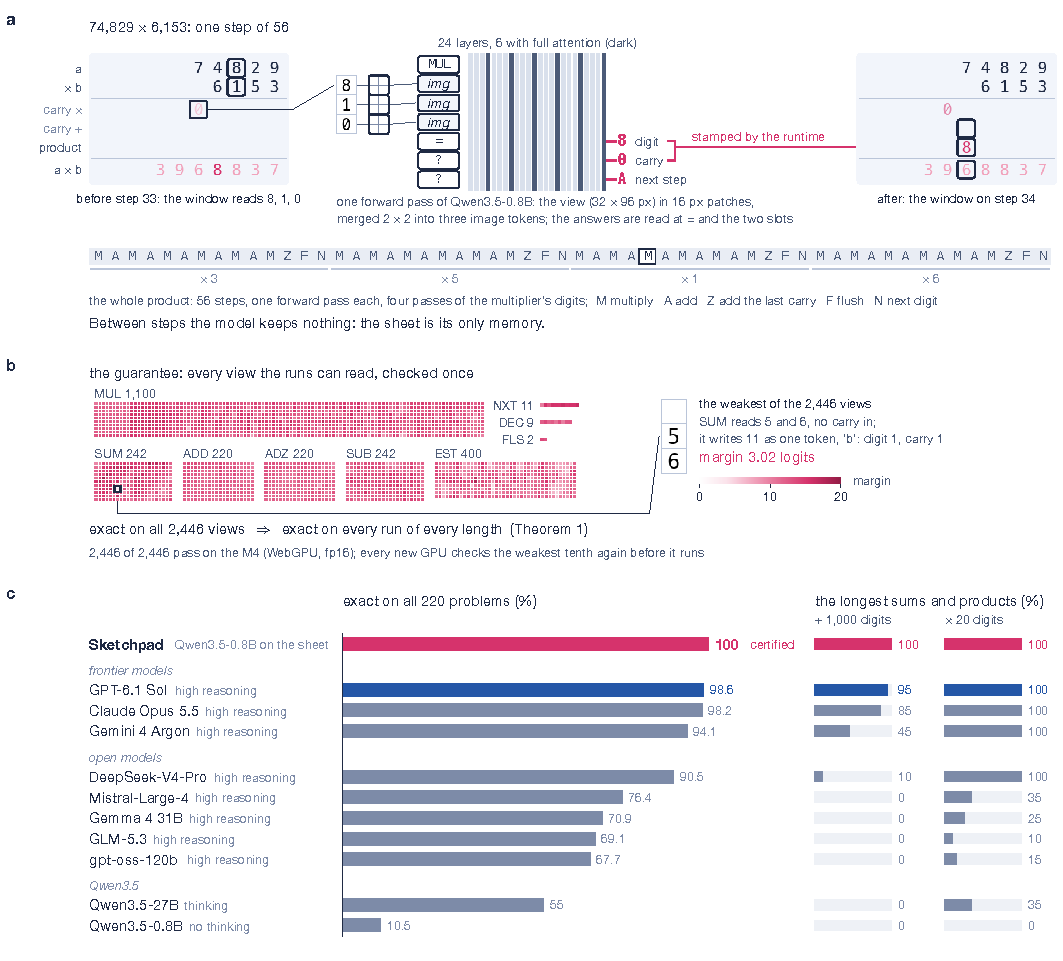
\includegraphics[width=\linewidth]{../figures/out/fig1.pdf}
\caption*{\textbf{Fig. 1 $|$} \textbf{The sheet: one step, any length, one certificate.} \textbf{a}, Long multiplication of 74,829 by 6,153 on the sheet, as the runtime lays it out, at step 33 of 56. The window (dark outline) shows the model three cells: a digit of each factor and the carry. What the model has written is in rose. \textbf{b}, One step is one forward pass of Qwen3.5-0.8B. The view, 32 × 96 pixels, enters the vision encoder as three image tokens after the step's word (\texttt{MUL}); the answers are read at \texttt{=\allowbreak{}} and at two placeholder slots: the digit, the carry and the next step (\texttt{A}, add the partial product). The 24 layers are 6 full-attention layers and 18 Gated DeltaNet layers. \textbf{c}, Share of problems answered exactly against digits per number: sums of 10 to 1,000 digits and products of 2- to 20-digit numbers, 20 problems per point (registered run, Methods). Sketchpad (rose) is exact on all 220; Qwen3.5-27B with chain of thought (cobalt) and Qwen3.5-0.8B with and without it (blue-grey) fall away with length. The certificate covers every length (dotted). \textbf{d}, The certificate: all 2,446 views, one square each, shaded by margin, as measured on the M4 in the browser. The smallest margin, 3.02 logits, is an addition view reading 5 and 6 with no carry.}\phantomsection\label{fig-sheet}
\end{figure}
\section{The sheet machine}\label{sec-machine}
\textbf{The model.} Qwen3.5-0.8B is an open vision-language model with a vision encoder and a 24-layer language model\cite{qwen35}. Six of its layers are full attention; the other eighteen are Gated DeltaNet layers, a form of linear attention that keeps a fixed-size running state instead of a cache of every past token\cite{yang2025gateddeltanet}. We add a LoRA adapter, a pair of small matrices beside each of 150 weight matrices of the language layers, whose product is added to the frozen weight's output\cite{hu2022lora}. The vision encoder and the base weights stay frozen.

\textbf{Views and steps.} The sheet is a grid of 32-pixel cells holding blank or a digit, drawn from one fixed set of glyph images. A view is a column of three cells, 32 × 96 pixels, which the vision encoder turns into three image tokens. A step is the prompt \texttt{WORD<image>=\allowbreak{}??}: a word naming the step (\texttt{SUM}, \texttt{MUL}, \texttt{ADD}, \texttt{SUB}, \texttt{EST}, \texttt{DEC} and four control words), the view, an equals sign and two placeholder slots. The model's answers are read at the equals sign and at the two slots of a single forward pass, so a step costs one pass however many answers it has (Fig. \hyperref[fig-sheet]{1}b). Because every layer of the model is causal, what follows the equals sign cannot change the answer read there, so every prompt is padded to the same length and steps of different kinds share one batch (Methods).

\textbf{Tables.} For each step word, the \emph{table} lists every view the step can meet with its correct answers. Column addition (\texttt{SUM}) reads a carry and two digits and writes their sum as one token, or \texttt{H} to halt: 242 views. Long multiplication uses five steps (multiply a digit pair with the carry, add into the running total, end a pass, flush the last carry, move to the next digit): 1,553 views. Subtraction (\texttt{SUB}, 242), guessing a quotient digit (\texttt{EST}, 400) and lowering a guess (\texttt{DEC}, 9) complete the calculator: 2,446 views in nine tables (Extended Data Table \hyperref[tbl-tables]{1}).

\textbf{The runtime.} The runtime is a small TypeScript program. For each procedure it lays the numbers out on the sheet, cuts the views, sends them to the model, writes the glyphs the model returns and moves the window as the model's next-step answer says. In multiplication it holds no arithmetic and no loop: the model's own next-step token decides when a row ends and when the product is done. In division and square roots the runtime chooses the procedure's skeleton (bring down the next digit, guess, multiply and subtract), and the branches inside it are the model's: the borrow the model writes out of the top column says whether a guess was too high. Every view the runtime cuts is checked against the tables before it is sent, and a view outside them would be reported; none occurred in any run reported here.

\textbf{Waves.} Independent procedures can share forward passes: when an algebra problem needs many separate products, the runtime steps them in lockstep and sends one view from each in a single batch. On the M4, a pass costs about 0.065 s plus 0.037 s per view in the batch, so batching cuts the fixed cost of a step, not the work per view (Fig. \hyperref[fig-machine]{2}c).

\begin{figure}[tbp]
\centering
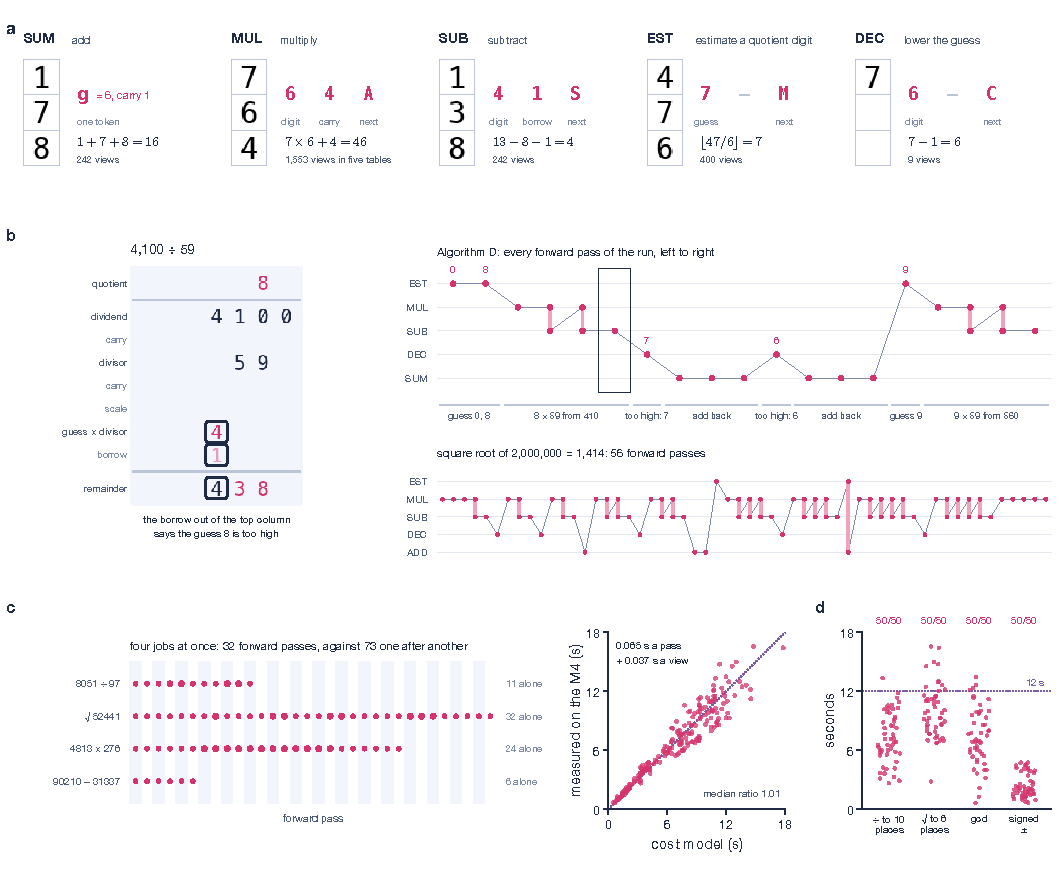
\includegraphics[width=\linewidth]{../figures/out/fig2.pdf}
\caption*{\textbf{Fig. 2 $|$} \textbf{The sheet machine.} \textbf{a}, The five step tables of the calculator, each with one real view (the model's own input pixels) and its answers in rose: \texttt{SUM} writes 6 with carry 1 from 1 + 7 + 8; \texttt{MUL} writes 6 and carry 4 from 7 × 6 + 4; \texttt{SUB} writes 4 and borrow 1 from 3 − 8 − 1; \texttt{EST} guesses 7 from ⌊47/6⌋; \texttt{DEC} lowers a guess of 7 to 6. \textbf{b}, A procedure is a walk over tables. Left, the division 4,100 ÷ 59 on its sheet, where the borrow out of the top column shows that the guess 8 is too high. Right, every forward pass of that run by Knuth's Algorithm D, and the 56 passes of the square root of 2,000,000. \textbf{c}, Waves: four independent jobs share 32 forward passes instead of 73 one after another. Measured seconds on the M4 against the cost model (0.065 s per pass plus 0.037 s per view) for the 200 registered problems; the median ratio is 1.01. \textbf{d}, The 200 registered problems in the browser, 50 per set, all exact; seconds per problem against the 12-second line.}\phantomsection\label{fig-machine}
\end{figure}
\section{Certification}\label{sec-cert}
\textbf{Margins.} The model's answer at a position is the token with the largest logit, the score the network gives each possible token. A view \emph{passes} when, at every answer position, the correct token's logit exceeds every other; the smallest difference is its \emph{margin}, and a margin of 3 makes the correct token about 20 times more probable than any other. A \emph{certificate} records that every view of every table passes, with the margins.

We certify twice. In PyTorch on the training server, in 32-bit floating point, the smallest margin over the 2,446 views is 3.96 (an addition view; Extended Data Table \hyperref[tbl-tables]{1}). In the browser, the page runs the deployed graph through ONNX Runtime Web on WebGPU\cite{onnxruntime,transformersjs,webgpu} in 16-bit floating point, in exactly the padded batch form that runs; on the M4 all 2,446 views pass, with smallest margins 3.02 for addition, 6.52 for the multiplier's steps and 4.61 for the calculator's (Fig. \hyperref[fig-cert]{3}c). The full check takes 3.5 minutes there. The certificate travels with the model files, fingerprinted by the hash of every file, and a visitor's GPU checks the weakest tenth of every table again, the rows with the smallest margins, before it trusts the shipped table; it can check all of them on request.

\textbf{What the certificate implies.} Write $C$ for the configurations of a procedure (the whole sheet, the window's place and the procedure's control state), $V$ for the views, and $A$ for the answers. At a configuration $c$ the runtime either halts or shows the model a view $v=\mathrm{view}(c)$, then paints the model's answer: $c' = \mathrm{paint}(c, f(v))$. Under the \emph{pinned-sheet policy}, each forward pass sees the step's prompt and its view and nothing else, so the model's answers are a function $f: V\to A$. The reference table is $T: V \to A$.

\begin{thmbox}\phantomsection\label{thm-p}\noindent\textbf{Theorem 1} (Theorem P, sheet form).\enspace\itshape Suppose the runtime paints the answer, so that different answers to a view give different sheets. Then for every start in a set $I$ and every number of steps, the model's run equals the reference run configuration by configuration if and only if $f(v) = T(v)$ for every view $v$ that some reference run from $I$ meets. In particular, if every such view is a row of the tables and the model passes every row, every run of every length is exact.\upshape

\noindent{\small\raggedright\textsc{Lean:} \texttt{Sketchpad.\allowbreak{}sheet\_\allowbreak{}exact\_\allowbreak{}iff}, \texttt{Sketchpad.\allowbreak{}sheet\_\allowbreak{}certified}, \texttt{Polyformer.\allowbreak{}Pinned.\allowbreak{}regeneration\_\allowbreak{}trace\_\allowbreak{}iff}, \texttt{Polyformer.\allowbreak{}Pinned.\allowbreak{}pinned\_\allowbreak{}regeneration\_\allowbreak{}iff}\par}
\end{thmbox}
\begin{proofbox}\noindent\textit{Proof sketch.}\enspace Sufficiency is induction on steps: if the two runs agree up to step $t$, they show the model the same view, which is a row the model passes, so they agree at step $t+1$. For necessity, take the first view where the model and the table disagree; the reference run meets it, and the two runs paint different answers there. The Lean proof instantiates the package's general regeneration theorem with the configuration as the state, so the sheet form and the token form of Theorem P are the same theorem.
\end{proofbox}
Theorem \hyperref[thm-p]{1} turns a statement about infinitely many runs into 2,446 checks, as Cai et al. did for learned recursive programs\cite{cai2017recursion} and Lewandowski et al. for a language model's decoding of a universal machine, by checking its 1,857 production rules\cite{lewandowski2026universal}. Its force lies in the hypothesis that the model's answer is a function of the view, which the pinned-sheet policy guarantees. If the model kept earlier steps in its context, as chain of thought does, no finite set of checks would suffice.

\begin{thmbox}\phantomsection\label{thm-nofinite}\noindent\textbf{Theorem 2} (No finite test once state leaves the sheet).\enspace\itshape Suppose each step's context keeps the earlier steps. Then for any finite set of test contexts there is a decoder, for a two-state table, that passes every row of the table and is right on every test context, all with strictly positive margins, and still makes an error on some longer run. The pinned run of the same decoder is exact at every length.\upshape

\noindent{\small\raggedright\textsc{Lean:} \texttt{Polyformer.\allowbreak{}Pinned.\allowbreak{}no\_\allowbreak{}finite\_\allowbreak{}test\_\allowbreak{}suite}, \texttt{Polyformer.\allowbreak{}Pinned.\allowbreak{}no\_\allowbreak{}finite\_\allowbreak{}check}\par}
\end{thmbox}
\begin{proofbox}\noindent\textit{Proof sketch.}\enspace The counterexample is a correct lookup plus one attention head whose write grows with the number of a given token in the context, scaled so that it crosses the margin only after more steps than any test contains. This is Moore's observation that no finite experiment identifies a machine whose number of states is unbounded\cite{moore1956gedanken}, realised by a decoder that passes the per-row certificate.
\end{proofbox}
Long procedures are built from many certified calls: a square root runs multiply-subtract passes, an algebra problem runs dozens of products and quotients whose inputs quote earlier results.

\begin{thmbox}\phantomsection\label{thm-compose}\noindent\textbf{Theorem 3} (Composition).\enspace\itshape Let a transcript make $K$ calls in order, each a certified procedure on its own sheet, whose inputs may quote the results of earlier calls. Every call's result equals its table's output on the input it actually received, at any lengths and in any order. If the final answer is wrong, then some table is wrong, some quote is wrong, or the glue that combines the results is wrong; for any distribution of transcripts, the probability of a wrong answer is at most the sum of the probabilities of those three events.\upshape

\noindent{\small\raggedright\textsc{Lean:} \texttt{Polyformer.\allowbreak{}Pinned.\allowbreak{}compose\_\allowbreak{}exact}, \texttt{Polyformer.\allowbreak{}Pinned.\allowbreak{}error\_\allowbreak{}decomposition\_\allowbreak{}certified}, \texttt{Polyformer.\allowbreak{}Pinned.\allowbreak{}error\_\allowbreak{}bound}\par}
\end{thmbox}
For the calculator the tables are fixed and correct by construction, so a wrong answer can come only from a wrong transcription of the problem or wrong glue. In the algebra of Section \hyperref[sec-algebra]{5}, the glue is the runtime's textbook procedure and every answer it returns is checked, so a wrong transcription is the remaining risk.

A certificate is measured on one code path: one device, one numerical precision, one batch shape. The run may take another.

\begin{thmbox}\phantomsection\label{thm-transfer}\noindent\textbf{Theorem 4} (Transfer across code paths).\enspace\itshape Suppose that at every view a run can meet, the logits on the path that runs differ from the certified logits by at most $\tau$ at every output. If every certified row has margin greater than $2\tau$, the run is exact on every input of every length.\upshape

\noindent{\small\raggedright\textsc{Lean:} \texttt{Polyformer.\allowbreak{}Pinned.\allowbreak{}sel\_\allowbreak{}eq\_\allowbreak{}of\_\allowbreak{}close}, \texttt{Polyformer.\allowbreak{}Pinned.\allowbreak{}regeneration\_\allowbreak{}of\_\allowbreak{}close}, \texttt{Polyformer.\allowbreak{}Pinned.\allowbreak{}policy\_\allowbreak{}tick\_\allowbreak{}eq}\par}
\end{thmbox}
\begin{proofbox}\noindent\textit{Proof sketch.}\enspace At each view the correct token leads by more than $2\tau$ on the certified path; moving every logit by at most $\tau$ cannot overturn that lead, so each step picks the same answer, and Theorem \hyperref[thm-p]{1} applies. The package also proves that a pinned step computed through a cached prompt prefix, with the step's tokens evicted after each step, gives the same logits as a fresh forward pass, so that choice of cache is another path with $\tau = 0$ in exact arithmetic.
\end{proofbox}
Theorem \hyperref[thm-transfer]{4} explains what we measured on hardware. A 4-bit quantised decoder moved some add rows of an earlier adapter from a margin of +9.4 on the server to −8.9 on the M4, far more than any margin, so the page ships the 16-bit decoder, which reproduces the server's certificate. Padding the addition prompt to the batch form moved no margin by more than 0.0018. The device certificate is measured on the path that runs, so there $\tau$ is only the variation between runs; two certificates taken on the M4, with and without the gate, agree on all 2,446 margins to the stored thousandth. On another GPU, the spot check of the weakest tenth measures how far the margins have moved (Fig. \hyperref[fig-cert]{3}d).

\begin{figure}[tbp]
\centering
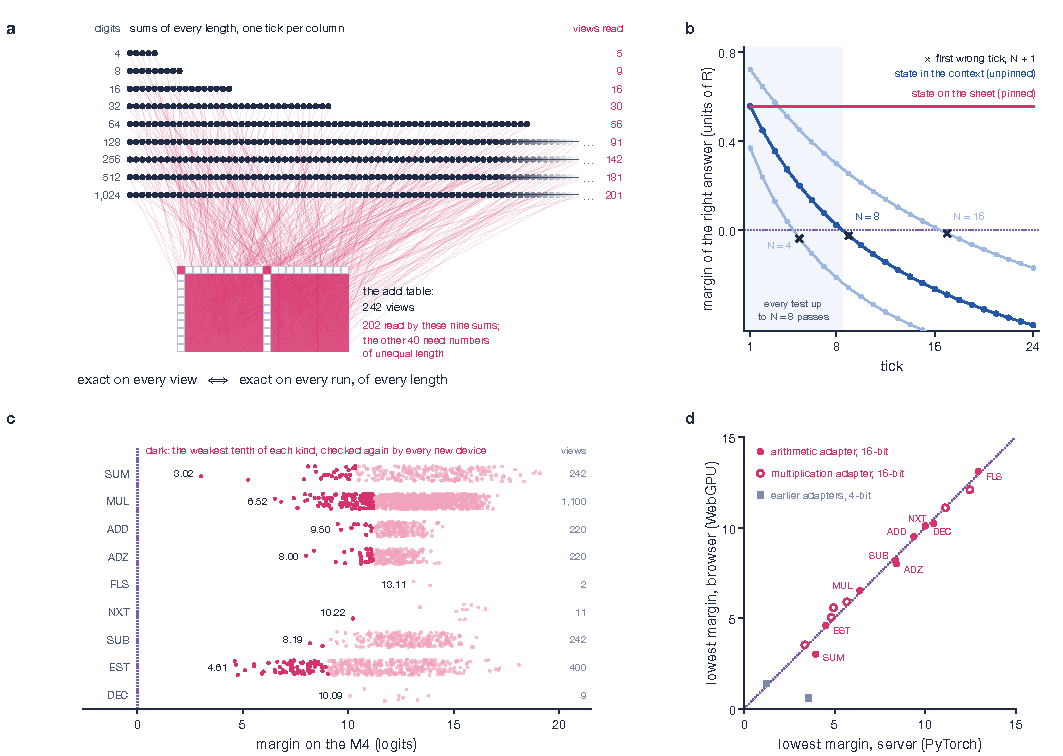
\includegraphics[width=\linewidth]{../figures/out/fig3.pdf}
\caption*{\textbf{Fig. 3 $|$} \textbf{Certification.} \textbf{a}, Sums of every length, one step per column, read only views from the 242-view addition table; nine sums from 4 to 1,024 digits already read 202 of them, and the other 40 need numbers of unequal length. Exact on every view is exact on every run (Theorem \hyperref[thm-p]{1}). \textbf{b}, The counterexample of Theorem \hyperref[thm-nofinite]{2}: when the state lives in the context, a decoder can pass every test up to $N$ steps and fail at step $N+1$ (blue, for $N$ = 4, 8 and 16), while the pinned run keeps its margin at every step (rose). \textbf{c}, Margins of all 2,446 views on the M4, per step word; the weakest tenth of each, which every new device checks again, is dark. \textbf{d}, Smallest margin per step word on the server (PyTorch, 32-bit) against the browser (WebGPU): the 16-bit decoder follows the identity line for the published model (E7) and the one before it (E6); the 4-bit decoder of the first adders (E2, E2b) moved the smallest margin by up to 3 logits.}\phantomsection\label{fig-cert}
\end{figure}
\section{A calculator on the sheet}\label{sec-calc}
Every key of a pocket calculator is a pen-and-paper procedure over a few digit tables. Signed sums and differences use addition or subtraction column by column; the borrow out of the last column says which number was larger, so the sign comes free. Multiplication is the schoolbook method, one multiply step per digit pair and one add step per partial-product digit.

\textbf{Division} follows Knuth's Algorithm D, the standard method for dividing long numbers\cite{knuth1997taocp2}. Both numbers are first scaled by a single digit so that the divisor's leading digit is at least 5, which costs one multiplication pass. Each quotient digit is then guessed from the top two digits of the remainder and the top digit of the divisor, the \texttt{EST} table. After scaling, the guess is never too small and at most two too large. The runtime multiplies the divisor by the guess and subtracts it from the remainder in one pass; if the model's borrow out of the top column is 1, the guess was too high, \texttt{DEC} lowers it and the divisor is added back.

\textbf{Square roots} are taken digit by digit, the method taught in schools, bringing the number down two digits at a time. We scale the number by $c^2$, with $c$ one of 1, 2, 4 or 5, so that the root starts with 25 to 49; twice the root then starts with 5 to 9, so each digit's guess is division's guess, at most two too high, and the same three tables serve. The \textbf{greatest common divisor} is Euclid's algorithm by repeated division.

We registered the test before running it: 50 problems each of division to 10 decimal places, square roots to 6 places, greatest common divisors of numbers up to 999, and signed sums and differences of up to 20 digits, run one after another in the browser on the M4. All 200 answers were exact, and every view of every run was a certified row. Median times were 7.0 s for division, 9.8 s for square roots, 7.0 s for the greatest common divisor and 2.0 s for sums (Fig. \hyperref[fig-machine]{2}d; Extended Data Table \hyperref[tbl-t3]{2}). 184 of 200 finished within 12 s; the slowest were roots of three-digit numbers, at up to 16.5 s, because the trial divisor grows a digit with every root digit and a guess that is too high costs a whole pass. Measured times followed the cost model with a median ratio of 1.01.

On a server GPU, where many problems can run in one batch, the same model answered all 220 problems of the registered baseline, sums of 10 to 1,000 digits and products of 2- to 20-digit numbers: 64,700 views, all certified rows, in 1,001 batched forward passes. Qwen3.5-27B with chain of thought, run with the same prompts and a 32,768-token budget, answered 121 of the 220, falling from 18 of 20 ten-digit sums to none of the thousand-digit ones and from 20 of 20 four-digit products to 7 of 20 twenty-digit ones; 93 of its 99 failures reached the token budget. Stock Qwen3.5-0.8B answered 3 of 220 with chain of thought, nearly always looping until the budget ran out, and 23 without (Fig. \hyperref[fig-sheet]{1}c; Extended Data Table \hyperref[tbl-baselines]{5}).

\section{Algebra as written}\label{sec-algebra}
Algebra in school is arithmetic organised by a few rewriting rules. The runtime writes a derivation the way a textbook would, one line per step, and every number on every line comes from a certified procedure on the sheet. To solve $3(x-2)+5=2x+14$, it multiplies out the bracket, which needs the product $3\cdot 2$; collects $-6+5$; moves the terms across; divides; and substitutes $x=15$ back into both sides, which gives 44 on each. Quadratics use the discriminant and the quadratic formula, with a square root that ends with remainder zero exactly when the roots are rational. Powers of a binomial are expanded by the binomial theorem, with Pascal's rule supplying the coefficients by addition. Polynomials are factored by the rational root theorem, which says that a rational root of an integer polynomial is a divisor of the constant term over a divisor of the leading coefficient, and by synthetic division, the shortcut for dividing by $x - r$; systems of equations by elimination (Fig. \hyperref[fig-algebra]{4}a). Irrational roots of quadratics are given exactly, as simplified radicals such as $3 \pm \sqrt 5$, checked through Vieta's formulas, that the roots sum to $-b/a$ and multiply to $c/a$, in integer arithmetic.

\textbf{Every answer is checked.} Rational roots are substituted back into the equation, expansions are compared with the original at a further point, and irrational root pairs pass the Vieta identities exactly; an answer that fails is refused and the failed check is shown. A substitution check confirms the roots found, not that all roots were found; the runtime knows the degree and reports when a factor remains unresolved. With deliberately planted faults, the checks refused 200 of 200 wrong roots offered as answers, and 185 of 200 runs in which one call's arithmetic was corrupted; in the 15 runs they did not refuse, the corrupted number did not change the answer (Fig. \hyperref[fig-algebra]{4}b). The certificate already covers the arithmetic; the checks guard what it does not cover, the runtime's algebra and the transcription of the problem, and as the planted faults show they also catch most arithmetic faults.

\textbf{Cost.} The algebra is classical and so is the comparison. Computer algebra can also solve by evaluating both sides at a few numbers and reading the polynomial off the values (interpolation\cite{kaltofen1990blackbox}), or by evaluating at a power of ten so the coefficients appear in groups of digits (Kronecker substitution\cite{kronecker1882}: $(x+2)^5$ at $x=1000$ is $1\,010\,040\,080\,080\,032$). That route needs only arithmetic too, but it hides the algebra and costs more rows on the sheet. By the cost model, which the calculator's measured times follow (median ratio 1.01), the textbook route takes 2.8 s for the linear equation above against 4.5 s by evaluation, 12.1 s for $(x+2)^5$ against 33.1 s, and 16.9 s to factor $x^3-6x^2+11x-6$ against 31.5 s. Six of the eleven worked examples take less than 12 s by the cost model, by either route and either check. Measured on the M4 with the default check, eight do: the expansions of $(x+2)^5$ and $(2x-3)^4$ finish in 9.5 and 10.4 s, while $(x+1)^{10}$, cubic factoring and a three-by-three system take 16 to 22 s. The exact irrational roots of three quadratics take 7.4 to 11.2 s, and their four-place decimal approximations, which the page shows after the exact answer, about as long again (Fig. \hyperref[fig-algebra]{4}c; Extended Data Table \hyperref[tbl-algebra]{3}).

\begin{figure}[tbp]
\centering
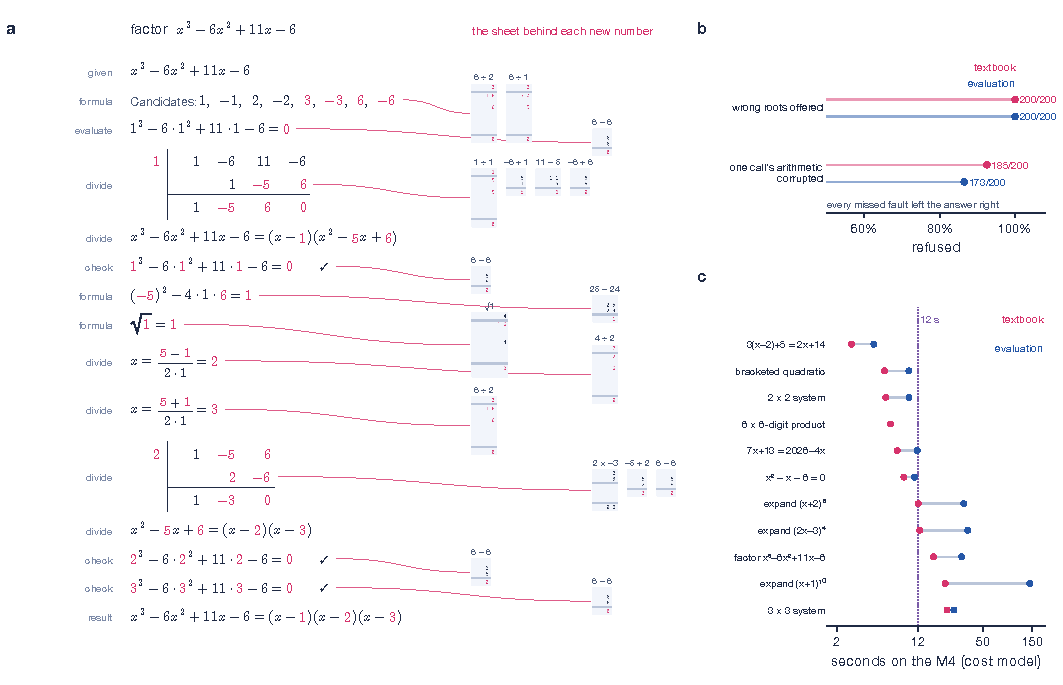
\includegraphics[width=\linewidth]{../figures/out/fig4.pdf}
\caption*{\textbf{Fig. 4 $|$} \textbf{Algebra as written.} \textbf{a}, Factoring $x^3-6x^2+11x-6$, typeset as the runtime writes it. Each number in rose was computed by the model on its sheet; the thread leads from the number to the small column sum or product that produced it. Numbers copied from the problem stay in ink. \textbf{b}, Refusals under planted faults: wrong roots offered as answers (200 of 200 refused by both routes) and one call's arithmetic corrupted (185 of 200 refused by the textbook route, 173 of 200 by evaluation); every fault that was not refused left the answer right. \textbf{c}, Seconds for eleven worked examples with the default check: the textbook route measured on the M4 (rose) and by the cost model (open rose), against evaluation and interpolation by the cost model (cobalt), with the 12-second line.}\phantomsection\label{fig-algebra}
\end{figure}
\section{One model that decides}\label{sec-gate}
Teaching a model a new skill tends to erode its old ones, the problem of continual learning\cite{mccloskey1989catastrophic,kirkpatrick2017ewc}. Our arithmetic adapters barely move the model's perplexity on plain text, the usual check: the multiplier adapter E6 raised it by a factor of 1.0065. Yet with that adapter on, the model's instruction following dropped by 16.4 points on IFEval, a benchmark of prompts with checkable instructions\cite{zhou2023ifeval}. Perplexity does not see the damage.

\textbf{The gate.} We therefore built the adapter into the graph behind a gate, in the spirit of progressive networks, which add capacity beside a frozen model instead of changing it\cite{rusu2016progressive}. Every adapter branch's output is multiplied by one input of the graph, $g$, before it is added back: $y = xW + g\,s\,(xA^{\top})B^{\top}$, where $W$ is the frozen weight, $A$ and $B$ the adapter's matrices and $s$ its fixed scale (Fig. \hyperref[fig-gate]{5}a). At $g=0$ every patched layer adds a floating-point zero, which returns the other operand unchanged, so the model is stock Qwen3.5-0.8B; at $g=1$ it is the sheet machine. On ONNX Runtime, over 2,500 chat forward passes and 2,688 table views, every logit, hidden state and cached state of the gated graph equals stock at $g=0$ and the ungated sheet machine at $g=1$, bit for bit, and greedy replies to all 100 chat prompts are identical. On the M4 the certificate at $g=1$ reproduced all 2,446 margins. The page's chat runs at $g=0$, so its language is stock by construction.

\textbf{Deciding to open the sheet.} The goal is a model that, in the middle of a reply, opens its sheet, writes a short work order, lets the certified procedures run, and continues with the results. That decision must live in weights that are on during chat, so the gate cannot provide it. We train it on synthetic dialogues (problems that need the sheet, distractors that do not, and problems inside prose) and score it on phrasings and scenarios held out from training. To keep the model's language, training adds a penalty on the divergence from the gate-0 model's own next-token distributions, on its replies to instruction prompts (self-distillation, as in Learning without Forgetting\cite{li2017lwf}) and on the model's own samples (on-policy distillation\cite{agarwal2024gkd,lu2025onpolicy}), the regime in which fine-tuning is known to forget least\cite{shenfeld2025razor}.

\begin{statusbox}\noindent\textbf{Today.}\enspace The fine-tune has not yet passed all of its registered bars. The best adapter so far opens the sheet on held-out problems with precision 1.000 and recall 0.991, keeps IFEval at stock (0.538 against 0.536; paired flips 52 won, 51 lost), writes correct work orders for 96\% of held-out equations, and keeps all 2,446 certified views and perplexity within 1\%. Three bars are still short: correct work orders for 85.6\% of held-out word problems against a bar of 90\%, and grade-school word problems (GSM8K\cite{cobbe2021gsm8k}) and general knowledge (MMLU\cite{hendrycks2021mmlu}) 2.4 and 2.2 points below stock against a bar of 2. Until all pass, the page's chat runs at the gate's stock setting.
\end{statusbox}
The runs so far show a trade-off. Each change that restored multi-step reasoning cost instruction following, until on-policy distillation removed most of that cost (Fig. \hyperref[fig-gate]{5}b). Opening the sheet is the easy part: stock Qwen, shown four examples, opens it with recall 0.81; the fine-tunes, shown none, with recall 0.946 to 0.998 (Fig. \hyperref[fig-gate]{5}c). The hard part is the language around it: translating a word problem into the right expression, which the sheet does not check.

\begin{figure}[tbp]
\centering
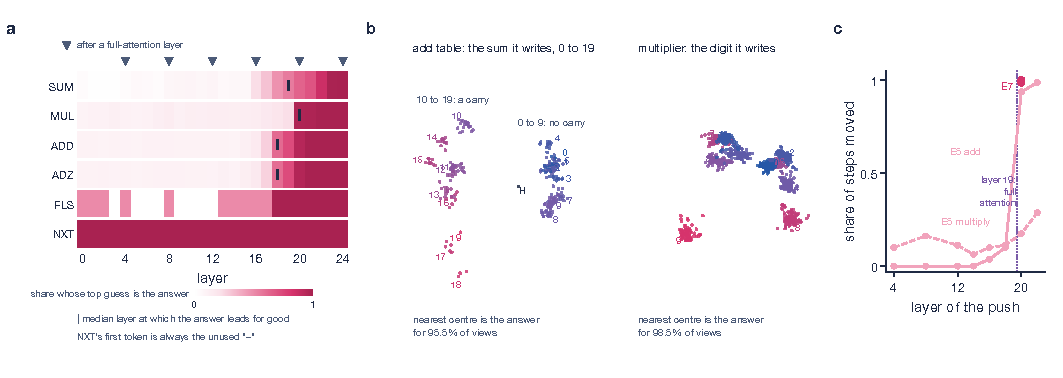
\includegraphics[width=\linewidth]{../figures/out/fig5.pdf}
\caption*{\textbf{Fig. 5 $|$} \textbf{One model that decides.} \textbf{a}, The gate: one input of the graph multiplies every adapter branch. At $g=0$ the model is stock Qwen3.5-0.8B bit for bit, on 2,500 chat forward passes and 2,688 table views; at $g=1$ it is the sheet machine. \textbf{b}, Instruction following (IFEval) against multi-step reasoning (GSM8K), in points against stock, for the chat fine-tunes P2 to P5 and for switching the gate inside a reply; the shaded region passes both bars. \textbf{c}, Opening the sheet on held-out problems: precision against recall, for stock Qwen with four examples (cobalt) and the fine-tunes (rose).}\phantomsection\label{fig-gate}
\end{figure}
\section{Inside the model}\label{sec-inside}
Where in the network is a step decided? The logit lens reads the residual stream, the running sum of every layer's output, through the model's final normalisation and output matrix after each layer, as if the network stopped there\cite{nostalgebraist2020logitlens,belrose2023tunedlens}. We count depth as the number of layers applied; the six full-attention layers end at depths 4, 8, 12, 16, 20 and 24. For the published model, the answer takes the lead for good at a median depth of 19 for addition, 20 for multiplication and 18 for the add steps of the multiplier, and through depth 15 it is the top token for at most 13\% of the views of any of these tables (Fig. \hyperref[fig-inside]{6}a).

The decision can be moved. A class-mean push adds to the residual stream, at the answer position, the difference between the mean state of a target answer and that of the true one\cite{turner2023actadd,rimsky2024caa}. Applied after depth 20, the end of the fifth full-attention layer, it changes 79 of 80 addition steps and 80 of 80 multiplication steps to the pushed answer. In an earlier adapter the same push moved 8 of 80 addition steps when applied after depth 18 and 75 of 80 after depth 20: the step is decided in or just before the full-attention layer that ends at depth 20 (Fig. \hyperref[fig-inside]{6}c). In a three-dimensional projection of the final layer, the states of the views gather by the answer they write, and the sums that carry (10 to 19) lie apart from those that do not (Fig. \hyperref[fig-inside]{6}b). The page runs this push on the visitor's own GPU, through an extra input of the graph, and shows the next step change.

\begin{figure}[tbp]
\centering
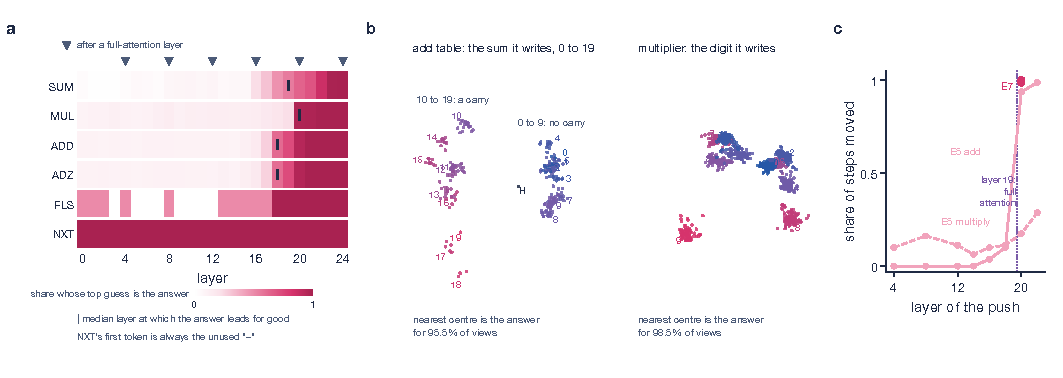
\includegraphics[width=\linewidth]{../figures/out/fig6.pdf}
\caption*{\textbf{Fig. 6 $|$} \textbf{Inside the model.} \textbf{a}, The logit lens: the share of views whose top token after each depth is the final answer, per step word; ticks mark the median depth at which the answer leads for good, triangles the ends of the full-attention layers. \textbf{b}, The states that write the answer, projected to three dimensions at the last layer and coloured by answer: addition (the sum written, 0 to 19) and the multiplier's digit. \textbf{c}, A class-mean push at the answer position: the share of steps changed to the pushed answer against the depth of the push, for an earlier adapter (E5, addition and multiplication) and the published one (E7, at depth 20).}\phantomsection\label{fig-inside}
\end{figure}
\section{Related work}\label{sec-related}
\textbf{Neural arithmetic.} Learned exact arithmetic at unbounded length has a long line. The Neural GPU learned binary addition and multiplication with convolutional updates that generalise far beyond training lengths\cite{kaiser2016neuralgpu}, with failures on structured inputs such as long runs of zeros\cite{price2016neuralgpu}. Arithmetic units with built-in inductive biases followed\cite{trask2018nalu,madsen2020nau}. For transformers, positional encodings and data formats decide whether addition generalises to longer inputs\cite{nogueira2021limitations,anil2022length,lee2024teaching,zhou2024raspl,zhou2024robust,mcleish2024abacus,cho2024coupling}, and fine-tuned language models reach near-perfect accuracy on bounded arithmetic\cite{liu2023goat,yang2023mathglm}, with division and the greatest common divisor the hard cases\cite{shen2024revorder,charton2024gcd,kasliwal2026division}. Neural cellular automata and differentiable transducers trained from scratch now add and multiply exactly at hundreds to thousands of times their training length\cite{wei2026nca,wei2026ncaadd,dfst2025}. Mechanistic studies find addition circuits that are correct on all but a vanishing fraction of inputs\cite{quirke2024verified}, and exactness has been proved for idealised training\cite{backdeluca2025exact}. Sketchpad differs in three ways: the executor is a pretrained vision-language model with a small adapter, not a network trained from scratch; its procedures include division, square roots and the greatest common divisor; and exactness is certified by exhausting the views, not estimated on samples.

\textbf{Procedures inside language models.} CAEF fine-tunes Llama-3.1-8B to step through arithmetic operators, division included, on a text tape, with one adapter per operator, reaching nearly 100\% up to 100 digits without a certificate\cite{lai2024caef}. OccamLLM and a gated calculator place exact arithmetic inside a language model as a built-in, non-learned module\cite{dugan2024occamllm,igc2025}; compiled and looped transformers run programs with hand-set weights\cite{giannou2023looped,loom2026,percepta2026vm,dong2023neuralcomprehension}; and a 60-million-parameter transformer trained as an interpreter predicts the steps of program traces thousands of lines long\cite{xu2026universal}. Chain of Code lets a language model emulate an interpreter for lines that cannot run\cite{li2024chainofcode}. In Sketchpad the procedure is learned, each step is one forward pass of a pretrained model, and nothing is carried between steps but the sheet.

\textbf{Tools.} Toolformer showed that a model can learn when to call a tool by keeping the calls that help\cite{schick2023toolformer}; PAL, Program of Thoughts, ToRA, ReTool and ToolRL interleave reasoning with code or tool calls\cite{gao2023pal,chen2023pot,gou2024tora,feng2025retool,qian2025toolrl}, and recursive language models call themselves through an interpreter\cite{zhang2025rlm}. Our chat fine-tune borrows Toolformer's recipe, with the model's own certified computation as the tool.

\textbf{Verification on finite sets.} Neural-network verification usually bounds a network's output over continuous regions of input\cite{katz2017reluplex}. Our inputs are finite by construction, so verification is enumeration. Moore showed that experiments on a machine identify it only given a bound on its states\cite{moore1956gedanken}, the basis of conformance testing\cite{chow1978testing}. Cai et al. proved learned recursive programs correct by checking a finite verification set\cite{cai2017recursion}. Schuurmans et al. and Lewandowski et al. certified universal computation by a language model's decoding by checking every production rule of a universal machine\cite{schuurmans2024universal,lewandowski2026universal}, Abbe et al. proposed the same context discipline, keeping the question and the current state and dropping the rest, as the inductive scratchpad\cite{abbe2024globality}, and PENCIL erases intermediate reasoning to keep the context short\cite{yang2025pencil}. Certification from examples can be hard under small changes of architecture, and length generalisation bounds can be uncomputable\cite{backdeluca2026certification,yang2026lengthbounds}; our guarantee needs no such bound, because the pinned-sheet policy makes the set of inputs finite. Our theorems are lifts of these results to a sheet; we claim the instance, its formal statement and its check on the deployed device.

\textbf{Reading rendered text.} Vision encoders can read text as pixels well enough to model language\cite{rust2023pixel,tschannen2023clippo,lee2023pix2struct}, and rendered text is now used to compress long contexts\cite{wei2025deepseekocr,cheng2025glyph}, though vision-language models that read digits reliably still fail at the multiplication\cite{balter2026vlm}. Visual scratch pads let multimodal models draw and reread diagrams as a visual chain of thought\cite{hu2024visualsketchpad,menon2024whiteboard,li2025mvot,selfimagine2024,mathcanvas2025}. Our sheet is narrower and exact: one fixed glyph set, read three cells at a time, where untouched Qwen3.5-0.8B reads single cells exactly but long rendered numbers only to 98 to 99\% per digit. The name Sketchpad nods to Sutherland's interactive drawing system\cite{sutherland1963sketchpad}.

\textbf{Algebra.} Transformers have learned symbolic integration\cite{lample2020symbolic}, step-by-step polynomial simplification with the arithmetic offloaded to a calculator\cite{agarwal2021polynomial}, Gröbner bases\cite{kera2024groebner} and, as large language models, school algebra in chain of thought\cite{lewkowycz2022minerva}; theory shows that chain of thought lets small transformers solve arithmetic and linear equations\cite{feng2023cot}. None is exact by construction. Our algebra algorithms are classical; what is new is that every number in them comes from a certified learned executor.

\textbf{Continual learning.} Learning without Forgetting distils the old model into the new one\cite{li2017lwf}; progressive networks keep the old weights and add new ones beside them\cite{rusu2016progressive}; elastic weight consolidation protects important weights\cite{kirkpatrick2017ewc}; X-LoRA routes between adapters\cite{buehler2024xlora}. On-policy distillation and RL's Razor show that forgetting tracks the divergence from the base on the model's own outputs\cite{agarwal2024gkd,lu2025onpolicy,shenfeld2025razor}. Our gate is a hard switch of the progressive kind: it guarantees stock behaviour at 0, and leaves the decision to compute to the fine-tune.

\textbf{What we did not find.} In a search of the literature on 30 October 2026, covering the work above and 50 arXiv abstracts read in full (Methods), we found no earlier pretrained vision-language model that does exact arithmetic at any length with a rendered sheet as its only state, certified on every view and checked again on the user's device; no learned, certified long division, square root or greatest common divisor; and no algebra whose every arithmetic step is done by a learned, certified executor.

\section{Limits}\label{sec-limits}
The certificate covers the model's steps and nothing else. The runtime's layout, its choice of procedure, and the transcription of a problem into a work order are not certified; they are ordinary code and, in chat, ordinary language. The theorems assume exact arithmetic; on hardware they hold through the margins, and the device certificate holds for the device and path that measured it. A visitor's GPU checks the weakest tenth of the shipped table, not all of it, unless asked. The algebra covers polynomial equations of small degree in one unknown and linear systems in up to three, and it checks the roots it finds, not that it found all of them. The model reads typed problems drawn in its own glyphs, not photographs. And it is slow: a step costs about 0.1 s on a laptop GPU, so a thousand-digit sum takes over a minute and some square roots and expansions take more than 12 s. The model that decides for itself when to compute is still in training.

\section*{Methods}\label{methods}
\subsection*{Model and adapter}
We use Qwen3.5-0.8B\cite{qwen35} (language model: 24 layers, hidden size 1,024; layers 4, 8, …, 24 are full attention with 8 query and 2 key-value heads, the rest Gated DeltaNet\cite{yang2025gateddeltanet}). The adapter is a LoRA of rank 16 and scale 32/16 on the query, key, value and output projections of the 6 attention layers, the input and output projections of the 18 Gated DeltaNet layers and the three projections of all 24 feed-forward blocks: 150 matrices and 10,223,616 parameters, against 873,438,784 in the base model with its vision encoder. For the browser the model is exported to ONNX: the token embedding in 4-bit, the vision encoder and the language model in 16-bit floating point; the adapter is folded into a 21 MB decoder graph that shares the base's external weights. Two extra graph inputs serve the page: the gate (\texttt{lora\_\allowbreak{}gate}, Section \hyperref[sec-gate]{6}) and a push vector added to the residual stream after depth 20 (Section \hyperref[sec-inside]{7}); one extra output returns the hidden states for the inside view.

\subsection*{Views, prompts and tables}
Glyphs are 32 × 32 pixel sprites of blank and the ten digits, rendered once and reused for every view, so every view the model can see is one of a finite set of exact images. A view stacks three cells into a 32 × 96 image, which the processor, set to its native size, turns into three image tokens. The prompt of a step is its word, the image, \texttt{=\allowbreak{}} and two \texttt{?} slots, padded with further \texttt{?} to the length of the longest word; the answers are read at \texttt{=\allowbreak{}} and the two slots. Extended Data Table \hyperref[tbl-tables]{1} lists the nine tables. The rows are exhaustive over each step's possible views: for example, \texttt{MUL} covers every digit or blank of the multiplicand, every digit of the multiplier and every carry from blank to 8 (11 × 10 × 10 = 1,100), and \texttt{EST} covers every remainder pair under every normalised divisor digit from 5 to 9 (400). That the procedures meet no other view follows from the layout and, for division and roots, from normalisation; it is also checked by the runtime on every step, and by the reference runtime on 1,000 random cases per procedure, with no view outside the tables.

\subsection*{Training}
Training reads the tables, not sampled problems: every step draws rows from each table, and the loss is cross-entropy plus a hinge that pushes every margin above 4, plus a penalty on the divergence from the base model's next-token distributions on plain text\cite{li2017lwf}. Every 100 steps the whole certificate is computed; rows with margins below 2 are replayed, and training stops when every row passes with margin at least 3. The published adapter, E7, continued from the adapter E6, which already passed the addition and multiplication tables, with the subtraction, guess and lowering tables added. It passed every row first at step 1,200 and stopped at step 1,600, after 19.8 minutes on one H100 GPU (about \$1.30), with the learning rate decaying on a cosine from $2\times10^{-4}$ to $2\times10^{-5}$. Its plain-text perplexity is 1.0048 times stock. End to end on the server it multiplied 20 of 20 four-digit, 10 of 10 six-digit and 5 of 5 ten-digit pairs and added 20 of 20 ten-digit, 5 of 5 hundred-digit and 2 of 2 thousand-digit pairs exactly.

\subsection*{Certification}
A margin is the correct token's logit minus the largest logit of any other token in the vocabulary of 248,320, at each answer position; a row passes when every answer position has a positive margin. The server certificate runs in PyTorch in 32-bit floating point. The device certificate runs the deployed files (transformers.js 4.2.0\cite{transformersjs}, ONNX Runtime Web on WebGPU) on an Apple M4, through the page's own code path and padded batch form, and records every margin together with the device, the library version, the hash of every file and the sprite sheet. The page accepts a shipped certificate only for identical files, and checks the weakest tenth of each table again on the visitor's GPU before a run. The certificate file format is described in Appendix B.

\subsection*{Procedures and timing}
Signed sums and differences run \texttt{SUM} or \texttt{SUB} column by column; a subtraction ends on a halt row that reports whether a borrow came out, in which case the subtraction runs the other way round and the sign flips. Long division follows Algorithm D\cite{knuth1997taocp2}: both numbers are scaled by $f = \lfloor 10/(d+1) \rfloor$, $d$ the divisor's leading digit, in one multiplication pass each; each quotient digit is guessed by \texttt{EST} from the remainder's top two digits and the divisor's top digit (or skipped when the guess is zero); a multiply-subtract pass runs \texttt{MUL} one column ahead of \texttt{SUB}, two views per call; a borrow out of the top column triggers \texttt{DEC} and an add-back with \texttt{SUM}. Square roots scale the radicand by $c^2$ with $c\in\{1,2,4,5\}$ so the root starts with 25 to 49, which we verified for every radicand from 1 to 999,999; the first guess is 4, the second 9 when the root starts with 2, and every later guess comes from \texttt{EST}. The runtime picks $f$, $c$ and the first two guesses from the leading digits it lays out; each guess is at least the true digit and is lowered only by a certified multiply-subtract and \texttt{DEC}, so these choices can cost steps but cannot change a digit. Greatest common divisors run Euclid's algorithm by repeated division. The cost model, fitted on batches of 1 to 32 rows on the M4 with layer states left on the GPU, is 0.065 s per forward pass plus 0.037 s per view.

The registered browser test (Extended Data Table \hyperref[tbl-t3]{2}) drew its 200 problems from a fixed generator (seed 12345) before any run: $a \div b$ to 10 places with $a \le 999$ and $2 \le b \le 99$; $\sqrt a$ to 6 places with $2\le a \le 999$; $\gcd(a,b)$ with $10 \le a,b \le 999$; and signed sums and differences of 1 to 20 digits. It ran in Chrome on an Apple M4 in the page's fast mode, one problem after another, with wall time measured from the call to the answer. The WebGPU device was lost three times during the run; each time the model was reloaded and the interrupted problem redone, and only completed runs are counted. Every answer was checked against the page's own big-integer arithmetic and again in Python. The run was repeated in full with the gated published model: all 200 answers were again exact, and every step's views and answers were identical.

\subsection*{Algebra}
The algebra runtime (\texttt{program/\allowbreak{}}) parses a problem, writes the derivation line by line, and obtains every number through the calculator's interface, which runs certified procedures on the sheet; independent calls share waves. Each line records which model calls produced its numbers, which the page uses to light each number when its call completes (Fig. \hyperref[fig-algebra]{4}a). The light check confirms collected coefficients at one further point and substitutes rational roots into the collected equation; the strong check substitutes into the typed sides. Irrational roots of a quadratic $ax^2+bx+c$ are written as a reduced pair $(p \pm q\sqrt m)/d$ and checked by the integer identities $a\cdot 2p = -b\,d$ and $a(p^2 - q^2 m) = c\,d^2$, which hold exactly when the pair is the quadratic's two roots; square factors are extracted by trial of the primes up to 50. The fault populations planted a wrong root (200 per route) or corrupted the result of one call inside the initial evaluation or collection work (200 per route, fixed seeds); a second population perturbed one parameter of 200 radical pairs, and all 200 were refused in both check modes. The reference test suite of 264 tests, including 2,200 generated problems per route and check mode, runs with exact reference tables in place of the model; every cost is computed by the cost model from rows and calls, not measured on the device.

\subsection*{The gate}
The gate multiplies each LoRA branch's output before it is added to the frozen projection, in all 150 patched matrices. The identity test ran on ONNX Runtime 1.31.1 on CPU, with three graphs on the same external weights: stock (the base with the inside patch), the ungated adapter and the gated one. It compared every logit, hidden state and cached state, bit for bit, on 100 chat prompts (the first user turn of the No Robots test split\cite{norobots2023}; one prefill and 24 greedy decoding steps each, 2,500 calls) and on all 2,446 table views plus the 242 addition views in padded form, with inputs captured from the reference forward pass.

\subsection*{The chat fine-tune}
The training set has about 3,150 synthetic dialogues, of which about 30\% are distractors that must not open the sheet, plus 547 grade-school training problems solved by stock Qwen in its own words, with each calculation turned into a sheet call and kept only when the stand-in sheet reproduced it. The held-out set has 780 items from templates never trained on. Every work order is scored by running it, never by string match. Registered bars, set before any run: precision and recall of opening the sheet at least 0.95; correct work orders for at least 90\% of word problems and 95\% of equations and expressions; IFEval strict prompt-level accuracy\cite{zhou2023ifeval} within 2 points of stock; and, from the second round, GSM8K (250 test problems) and MMLU (500 questions) within 2 points of stock. Kill lines: any certified view lost, perplexity above 1.03 times stock, or IFEval more than 5 points down. Paired flips (the prompts only one of two models gets right) give the noise of each comparison. Extended Data Table \hyperref[tbl-chat]{4} lists every run.

\subsection*{Inside the model}
The logit lens applies the final normalisation and output matrix to the residual stream after each depth at the first answer position, for the 1,795 addition and multiplication views; a view's decision depth is the first depth after which the final answer stays the top token. The class-mean push replaces the answer position's state after depth 20 by itself plus the mean state of the target answer's views minus the mean of the true answer's, and counts how often the step's answer becomes the target (80 trials per table).

\subsection*{Baselines}
The baseline of Fig. \hyperref[fig-sheet]{1}c was registered before it ran (\texttt{paper/\allowbreak{}BASELINES.\allowbreak{}md}): 220 problems, 20 per length, sums of 10, 30, 100, 300 and 1,000 digits and products of 2-, 4-, 6-, 10-, 15- and 20-digit numbers (seed 20261031), the same prompt for every model (``What is a + b? Give the exact integer. Put the final answer in \textbackslash{}boxed\{\}.''), Qwen's recommended sampling for each mode, and a budget of 32,768 new tokens with chain of thought and 4,096 without. The stock models ran under vLLM on one H100 GPU. The 27-billion-parameter slot used the FP8 release of Qwen3.5-27B, because the 16-bit model held only 8 replies at full length and would have exceeded the budget; the choice was fixed before scoring. Sketchpad ran in PyTorch with the published adapter, all 220 problems in lockstep. The answer was the last boxed integer after the reasoning, separators removed; a reply that hit the budget or gave no answer counted as wrong. The run cost about \$7 on Modal.

\subsection*{Literature search}
The prior-art search of 30 October 2026 read 50 arXiv abstracts and the proof method of Cai et al., on exact arithmetic by learned models, certification of learned programs, procedure-stepping and compiled arithmetic in language models, algebra by learned models, tool use and adapter switching. It is a search, not a proof of absence. Every reference in this paper was checked against its source on 31 October 2026 (\texttt{paper/\allowbreak{}refs\_\allowbreak{}verified.\allowbreak{}md}).

\subsection*{Data and code availability}
The model, its adapter, the certificate and the inside data are on Hugging Face (\texttt{mohsenvand/\allowbreak{}sketchpad-0.\allowbreak{}8b-preview}, revision \texttt{2df87172}). The runtime, the page, the algebra, the baselines and this paper's sources are in the Sketchpad repository under the Apache 2.0 licence. The training and evaluation scripts and the records cited in \texttt{paper/\allowbreak{}numbers.\allowbreak{}md} are in the polyformer repository (\texttt{research/\allowbreak{}sketch/\allowbreak{}}) and in this one. The Lean proofs are in the polyformer package \texttt{research/\allowbreak{}lean} (branch \texttt{lean-p}) and in \texttt{paper/\allowbreak{}lean/\allowbreak{}Sheet.\allowbreak{}lean}.

\section*{Extended Data}\label{extended}
\begin{table}[tbp]
\centering
\caption*{\textbf{Extended Data Table 1 $|$} \textbf{The nine tables.} Each row is one view the step can meet. Margins are the smallest over the table, in logits, for the published model: on the server in 32-bit PyTorch, and on the M4 in the browser in 16-bit, from the shipped certificate. Next-step letters: \texttt{A} add the partial product, \texttt{Z} end of pass, \texttt{M} multiply (or multiply-subtract), \texttt{F} flush, \texttt{N} next digit, \texttt{H} halt, \texttt{B} borrow out, \texttt{S} subtract on, \texttt{C} correct the remainder.}\phantomsection\label{tbl-tables}
{\small
\begin{tabularx}{\linewidth}{l>{\raggedright\arraybackslash}X>{\raggedright\arraybackslash}Xrrr}
\toprule
Step & View (top to bottom) & Answers at \texttt{=\allowbreak{}}, \texttt{?}, \texttt{?} & Rows & Server & M4 \\
\midrule
\texttt{SUM} & carry (blank, 1), top digit, bottom digit (blank, 0–9) & sum and carry as one token (0–19), or \texttt{H} & 242 & 3.96 & 3.02 \\
\texttt{MUL} & multiplicand digit (blank, 0–9), multiplier digit (0–9), carry (blank, 0–8) & digit, carry, \texttt{A} or \texttt{Z} & 1,100 & 6.39 & 6.52 \\
\texttt{ADD} & carry (blank, 1), product digit, running-total digit (blank, 0–9) & digit, carry, \texttt{M} & 220 & 9.37 & 9.50 \\
\texttt{ADZ} & as \texttt{ADD}, at the end of a pass & digit, carry, \texttt{F} & 220 & 8.41 & 8.00 \\
\texttt{FLS} & carry (blank, 1), blank, blank & the last carry, –, \texttt{N} & 2 & 12.93 & 13.11 \\
\texttt{NXT} & next multiplier digit (blank, 0–9), blank, blank & –, –, \texttt{M} or \texttt{H} & 11 & 10.48 & 10.22 \\
\texttt{SUB} & borrow (blank, 1), top digit, bottom digit (blank, 0–9) & digit, borrow, \texttt{S}; all blank: –, –, \texttt{H} or \texttt{B} & 242 & 8.36 & 8.19 \\
\texttt{EST} & remainder's top two digits $r_1 \le d$, divisor's top digit $d$ (5–9) & $\min(9, \lfloor(10r_1+r_2)/d\rfloor)$, –, \texttt{M} or \texttt{N} & 400 & 4.51 & 4.61 \\
\texttt{DEC} & guess $q$ (1–9), blank, blank & $q-1$, –, \texttt{C} & 9 & 10.00 & 10.09 \\
\textbf{All} &  &  & \textbf{2,446} & \textbf{3.96} & \textbf{3.02} \\
\bottomrule
\end{tabularx}
}
\end{table}
\begin{table}[tbp]
\centering
\caption*{\textbf{Extended Data Table 2 $|$} \textbf{The registered browser test.} 50 problems per set on the Apple M4 (WebGPU, 16-bit decoder), ungated E7; the full certificate passed first.}\phantomsection\label{tbl-t3}
{\small
\begin{tabularx}{\linewidth}{>{\raggedright\arraybackslash}Xrrrrrr}
\toprule
Set & Exact & Median s & Max s & Over 12 s & Median calls / views & Cost model median s \\
\midrule
$a \div b$ to 10 places ($a \le 999$, $b \le 99$) & 50 & 7.0 & 13.3 & 1 & 65 / 90 & 7.6 \\
$\sqrt a$ to 6 places ($a \le 999$) & 50 & 9.8 & 16.5 & 11 & 86 / 137 & 10.7 \\
$\gcd(a,b)$ ($a, b \le 999$) & 50 & 7.0 & 13.4 & 4 & 61 / 84 & 7.1 \\
signed $\pm$, up to 20 digits & 50 & 2.0 & 4.7 & 0 & 19 / 19 & 1.9 \\
\bottomrule
\end{tabularx}
}
\end{table}
\begin{table}[tbp]
\centering
\caption*{\textbf{Extended Data Table 3 $|$} \textbf{Cost of the worked algebra examples.} Rows (views), forward passes after waves and seconds by the cost model, light check, for the textbook and evaluation routes.}\phantomsection\label{tbl-algebra}
{\small
\begin{tabularx}{\linewidth}{>{\raggedright\arraybackslash}Xrr}
\toprule
Work order & Textbook rows / passes / s & Evaluation rows / passes / s \\
\midrule
\texttt{solve 3(x-2)+5=\allowbreak{}2x+14} & 36 / 22 / 2.8 & 75 / 27 / 4.5 \\
\texttt{solve 7x+13=\allowbreak{}2026-4x} & 97 / 62 / 7.6 & 165 / 88 / 11.8 \\
\texttt{solve 2x+3y=\allowbreak{}7,\allowbreak{} x-y=\allowbreak{}1} & 75 / 48 / 5.9 & 194 / 41 / 9.8 \\
\texttt{solve (2x-3)(x+5)=\allowbreak{}x\textasciicircum{}2+1-16} & 79 / 43 / 5.7 & 177 / 50 / 9.8 \\
\texttt{solve x\textasciicircum{}2-x-6=\allowbreak{}0} & 102 / 77 / 8.8 & 162 / 79 / 11.1 \\
\texttt{123456 * 654321} & 96 / 46 / 6.5 & 96 / 46 / 6.5 \\
\texttt{expand (x+2)\textasciicircum{}5} & 159 / 95 / 12.1 & 458 / 248 / 33.1 \\
\texttt{expand (2x-3)\textasciicircum{}4} & 172 / 94 / 12.5 & 492 / 274 / 36.0 \\
\texttt{factor x\textasciicircum{}3-6x\textasciicircum{}2+11x-6} & 195 / 149 / 16.9 & 483 / 210 / 31.5 \\
\texttt{expand (x+1)\textasciicircum{}10} & 322 / 154 / 21.9 & 2,359 / 845 / 142.2 \\
\texttt{solve 2x+3y-z=\allowbreak{}1,\allowbreak{} x-y+2z=\allowbreak{}3,\allowbreak{} 3x+y+z=\allowbreak{}8} & 323 / 167 / 22.8 & 538 / 102 / 26.5 \\
\texttt{solve x\textasciicircum{}2-2=\allowbreak{}0} (exact answer) & 86 / 65 / 7.4 &  \\
\texttt{solve 2x\textasciicircum{}2+3x-1=\allowbreak{}0} (exact answer) & 144 / 88 / 11.0 &  \\
\texttt{solve x\textasciicircum{}2-6x+4=\allowbreak{}0} (exact answer) & 133 / 96 / 11.2 &  \\
\bottomrule
\end{tabularx}
}
\end{table}
\begin{table}[tbp]
\centering
\caption*{\textbf{Extended Data Table 4 $|$} \textbf{The chat fine-tunes against their registered bars.} Held-out templates at gate 1 with no examples, against stock Qwen with four examples (opening and work orders) or stock with none (benchmarks). IFEval, GSM8K and MMLU are in points against stock (0.536, 0.516 and 0.476). Bars as registered; GSM8K and MMLU became bars in the second round. P7 is running.}\phantomsection\label{tbl-chat}
{\small
\footnotesize\setlength{\tabcolsep}{3pt}
\begin{tabular}{llrrrrrrr}
\toprule
Run & Precision / recall & Word & Equations & Prose & IFEval & GSM8K & MMLU & Views kept \\
\midrule
bar & ≥ 0.95 / ≥ 0.95 & ≥ 0.90 & ≥ 0.95 & ≥ 0.95 & ≥ −2 & ≥ −2 & ≥ −2 & all \\
stock, four examples & 0.971 / 0.809 & 0.789 & 0.583 & 0.667 & 0 & 0 & 0 &  \\
P1 (from E6) & 0.957 / 0.996 & 0.872 & 0.967 & 0.983 & −4.8 &  & −6.6 & 1,795 \\
P2 & 1.000 / 0.998 & 0.894 & 0.975 & 1.000 & −0.55 & −31.2 & −5.4 & 2,446 \\
P3 & 1.000 / 0.994 & 0.856 & 0.975 & 0.992 & −2.8 & −14.0 & −2.4 & 2,446 \\
P4 & 1.000 / 0.994 & 0.817 & 0.958 & 0.992 & −4.4 & −6.4 & −3.4 & 2,446 \\
P5 (on-policy) & 1.000 / 0.946 & 0.678 & 0.958 & 0.983 & −1.5 & −2.0 & −2.2 & 2,446 \\
P6 (wider word data) & 1.000 / 0.991 & 0.856 & 0.958 & 0.975 & +0.2 & −2.4 & −2.2 & 2,446 \\
\bottomrule
\end{tabular}
}
\end{table}
\begin{table}[tbp]
\centering
\caption*{\textbf{Extended Data Table 5 $|$} \textbf{The registered baseline.} Problems answered exactly, of 20 per cell, with the number of replies that reached the token budget in brackets. Qwen3.5-27B is the FP8 release.}\phantomsection\label{tbl-baselines}
{\small
\footnotesize\setlength{\tabcolsep}{3pt}
\begin{tabularx}{\linewidth}{>{\raggedright\arraybackslash}Xrrrrrrrrrrrr}
\toprule
System & +10 & +30 & +100 & +300 & +1,000 & ×2 & ×4 & ×6 & ×10 & ×15 & ×20 & All \\
\midrule
Sketchpad & 20 & 20 & 20 & 20 & 20 & 20 & 20 & 20 & 20 & 20 & 20 & 220 \\
Qwen3.5-27B, thinking & 18 (2) & 12 (8) & 8 (10) & 1 (19) & 0 (20) & 20 (0) & 20 (0) & 15 (4) & 14 (6) & 6 (11) & 7 (13) & 121 \\
Qwen3.5-0.8B, thinking & 0 (20) & 0 (20) & 0 (20) & 0 (20) & 0 (20) & 3 (17) & 0 (20) & 0 (20) & 0 (20) & 0 (20) & 0 (20) & 3 \\
Qwen3.5-0.8B, no thinking & 0 (8) & 0 (20) & 0 (20) & 0 (20) & 0 (20) & 15 (4) & 8 (9) & 0 (14) & 0 (20) & 0 (19) & 0 (20) & 23 \\
\bottomrule
\end{tabularx}
}
\end{table}
\appendix
\section*{The Lean package}\label{app-lean}
The theorems are proved in Lean 4\cite{demoura2021lean4} with Mathlib\cite{mathlib2020} (Lean and Mathlib 4.35.0). The package builds with \texttt{lake build} (3,150 jobs) and contains no \texttt{sorry}, \texttt{admit} or added axiom; \texttt{\#print axioms} on every theorem below lists only \texttt{propext}, \texttt{Classical.\allowbreak{}choice} and \texttt{Quot.\allowbreak{}sound}, Lean's standard axioms, or a subset. The model in Lean is an abstraction: the network is a deterministic function of its context (or a causal decoder whose layer at a position reads only earlier positions), the argmax may break ties any way, and arithmetic is exact; floating point enters only through Theorem \hyperref[thm-transfer]{4}`s $\tau$.

\begin{table}[tbp]
\centering
\caption*{\textbf{Extended Data Table 6 $|$} \textbf{Lean statements.} Files in the polyformer package \texttt{research/\allowbreak{}lean/\allowbreak{}Polyformer/\allowbreak{}} (branch \texttt{lean-p}, commit \texttt{a114d08b}), except \texttt{Sheet.\allowbreak{}lean}, which is \texttt{paper/\allowbreak{}lean/\allowbreak{}Sheet.\allowbreak{}lean} in this repository and builds against the package.}\phantomsection\label{tbl-lean}
{\small
\begin{tabularx}{\linewidth}{>{\raggedright\arraybackslash}X>{\raggedright\arraybackslash}Xll}
\toprule
Theorem & Lean name & File & Axioms \\
\midrule
\hyperref[thm-p]{1}, sheet form & \texttt{Sketchpad.\allowbreak{}sheet\_\allowbreak{}exact\_\allowbreak{}iff}, \texttt{Sketchpad.\allowbreak{}sheet\_\allowbreak{}certified} & \texttt{Sheet.\allowbreak{}lean} & \texttt{propext}, \texttt{Quot.\allowbreak{}sound} \\
\hyperref[thm-p]{1}, token form & \texttt{pinned\_\allowbreak{}regeneration\_\allowbreak{}iff}, \texttt{regeneration\_\allowbreak{}trace\_\allowbreak{}iff}, \texttt{pinned\_\allowbreak{}regeneration\_\allowbreak{}decoder} & \texttt{Pinned.\allowbreak{}lean} & standard \\
\hyperref[thm-nofinite]{2} & \texttt{no\_\allowbreak{}finite\_\allowbreak{}test\_\allowbreak{}suite}, \texttt{no\_\allowbreak{}finite\_\allowbreak{}check} & \texttt{Unpinned.\allowbreak{}lean} & standard \\
\hyperref[thm-compose]{3} & \texttt{compose\_\allowbreak{}exact}, \texttt{error\_\allowbreak{}decomposition\_\allowbreak{}certified}, \texttt{error\_\allowbreak{}bound} & \texttt{Compose.\allowbreak{}lean} & standard \\
\hyperref[thm-transfer]{4} & \texttt{sel\_\allowbreak{}eq\_\allowbreak{}of\_\allowbreak{}close}, \texttt{regeneration\_\allowbreak{}of\_\allowbreak{}close} & \texttt{Pinned.\allowbreak{}lean} & standard \\
\hyperref[thm-transfer]{4}, the cache & \texttt{policy\_\allowbreak{}tick\_\allowbreak{}eq}, \texttt{policy\_\allowbreak{}regeneration} & \texttt{Policy.\allowbreak{}lean} & \texttt{propext}, \texttt{Quot.\allowbreak{}sound} \\
\bottomrule
\end{tabularx}
}
\end{table}
\section*{The certificate format}\label{app-cert}
A certificate is one JSON file shipped beside the model graph (\texttt{arithmetic/\allowbreak{}certificate.\allowbreak{}json}). Its \texttt{format} string names the prompt forms it was measured in (for the published model, the padded addition prompt and the slotted, padded multiplier and calculator prompts, on 32 × 96 strips from the sprite sheet). It records the numerical precision of each graph, the transformers.js version, a fingerprint of the sprite sheet and of every model file, the device's GPU description and the time. For each table it lists the number of rows, the number that passed and every row's margin, in the table's fixed row order, to a thousandth of a logit. The page accepts it only if every fingerprint matches the files it loaded, and then checks the rows with the smallest tenth of margins again on the visitor's GPU.

\section*{Reproducing the numbers}\label{app-repro}
Every number in this paper is listed in \texttt{paper/\allowbreak{}numbers.\allowbreak{}md} with the record it comes from. Training, certification on the server, the identity test of the gate and the chat runs are Modal jobs in polyformer \texttt{research/\allowbreak{}sketch/\allowbreak{}} (\texttt{e7\_\allowbreak{}calc.\allowbreak{}py}, \texttt{e7\_\allowbreak{}gate\_\allowbreak{}identity.\allowbreak{}py}, \texttt{chat/\allowbreak{}}), each logged with its job id and cost. The device certificate and the registered browser test run on the page itself (\texttt{sketchpad.\allowbreak{}exportCertificate()} and \texttt{sketchpad.\allowbreak{}runCalc()} in the browser console). The algebra's tests and costs run with \texttt{pnpm vitest run src/\allowbreak{}lib/\allowbreak{}sketchpad/\allowbreak{}program}, and the costs are checked independently by \texttt{verify\_\allowbreak{}costs.\allowbreak{}py} and \texttt{verify\_\allowbreak{}round3.\allowbreak{}py}. The baseline is \texttt{paper/\allowbreak{}baselines/\allowbreak{}} (\texttt{spawn.\allowbreak{}py} launches it, \texttt{score.\allowbreak{}py} rebuilds \texttt{results.\allowbreak{}json} from the raw replies). The Lean proofs build as described above.

\section*{References}
\begingroup\small
\renewcommand{\refname}{}
\vspace{-2.5em}
\begin{thebibliography}{93}
\setlength{\itemsep}{1pt}
\bibitem{wei2022cot} Wei, J. et al. Chain-of-Thought Prompting Elicits Reasoning in Large Language Models. In Advances in Neural Information Processing Systems, 24824–24837 (2022). \url{https://arxiv.org/abs/2201.11903}
\bibitem{nye2021scratchpad} Nye, M. et al. Show Your Work: Scratchpads for Intermediate Computation with Language Models. Preprint at arXiv:2112.00114 (2021). \url{https://arxiv.org/abs/2112.00114}
\bibitem{nogueira2021limitations} Nogueira, R., Jiang, Z. \& Lin, J. Investigating the Limitations of Transformers with Simple Arithmetic Tasks. Preprint at arXiv:2102.13019 (2021). \url{https://arxiv.org/abs/2102.13019}
\bibitem{anil2022length} Anil, C. et al. Exploring Length Generalization in Large Language Models. In Advances in Neural Information Processing Systems, 38546–38556 (2022). \url{https://arxiv.org/abs/2207.04901}
\bibitem{lee2024teaching} Lee, N., Sreenivasan, K., Lee, J. D., Lee, K. \& Papailiopoulos, D. Teaching Arithmetic to Small Transformers. In International Conference on Learning Representations (ICLR 2024) (2024). \url{https://arxiv.org/abs/2307.03381}
\bibitem{zhou2024raspl} Zhou, H. et al. What Algorithms can Transformers Learn? A Study in Length Generalization. In International Conference on Learning Representations (ICLR 2024) (2024). \url{https://arxiv.org/abs/2310.16028}
\bibitem{zhou2024robust} Zhou, Y. et al. Transformers Can Achieve Length Generalization But Not Robustly. Preprint at arXiv:2402.09371 (2024). \url{https://arxiv.org/abs/2402.09371}
\bibitem{mcleish2024abacus} McLeish, S. et al. Transformers Can Do Arithmetic with the Right Embeddings. In Advances in Neural Information Processing Systems, 108012–108041 (2024). \url{https://doi.org/10.52202/079017-3430}
\bibitem{cho2024coupling} Cho, H. et al. Position Coupling: Improving Length Generalization of Arithmetic Transformers Using Task Structure. In Advances in Neural Information Processing Systems, 22233–22315 (2024). \url{https://doi.org/10.52202/079017-0701}
\bibitem{schick2023toolformer} Schick, T. et al. {Toolformer}: Language Models Can Teach Themselves to Use Tools. In Advances in Neural Information Processing Systems, 68539–68551 (2023). \url{https://doi.org/10.52202/075280-2997}
\bibitem{gao2023pal} Gao, L. et al. {PAL}: Program-aided Language Models. In Proceedings of the 40th International Conference on Machine Learning, 10764–10799 (2023). \url{https://arxiv.org/abs/2211.10435}
\bibitem{chen2023pot} Chen, W., Ma, X., Wang, X. \& Cohen, W. W. Program of Thoughts Prompting: Disentangling Computation from Reasoning for Numerical Reasoning Tasks. Transactions on Machine Learning Research (2023). \url{https://arxiv.org/abs/2211.12588}
\bibitem{gou2024tora} Gou, Z. et al. {ToRA}: A Tool-Integrated Reasoning Agent for Mathematical Problem Solving. In International Conference on Learning Representations (ICLR 2024) (2024). \url{https://arxiv.org/abs/2309.17452}
\bibitem{feng2025retool} Feng, J. et al. {ReTool}: Reinforcement Learning for Strategic Tool Use in {LLMs}. In International Conference on Learning Representations (ICLR 2026) (2026). \url{https://arxiv.org/abs/2504.11536}
\bibitem{moore1956gedanken} Moore, E. F. {Gedanken-Experiments} on Sequential Machines. In Automata Studies, 129–153 (1956). \url{https://doi.org/10.1515/9781400882618-006}
\bibitem{cai2017recursion} Cai, J., Shin, R. \& Song, D. Making Neural Programming Architectures Generalize via Recursion. In International Conference on Learning Representations (ICLR 2017) (2017). \url{https://arxiv.org/abs/1704.06611}
\bibitem{lewandowski2026universal} Lewandowski, A., Machado, M. C. \& Schuurmans, D. Universal computation is intrinsic to language model decoding. Preprint at arXiv:2601.08061 (2026). \url{https://arxiv.org/abs/2601.08061}
\bibitem{qwen35} {Qwen Team}. {Qwen3.5}: Towards Native Multimodal Agents. Qwen blog (2026). \url{https://qwen.ai/blog?id=qwen3.5}
\bibitem{hu2022lora} Hu, E. J. et al. {LoRA}: Low-Rank Adaptation of Large Language Models. In International Conference on Learning Representations (ICLR 2022) (2022). \url{https://arxiv.org/abs/2106.09685}
\bibitem{yang2025gateddeltanet} Yang, S., Kautz, J. \& Hatamizadeh, A. Gated Delta Networks: Improving {Mamba2} with Delta Rule. In International Conference on Learning Representations (ICLR 2025) (2025). \url{https://arxiv.org/abs/2412.06464}
\bibitem{onnxruntime} {ONNX Runtime developers}. {ONNX Runtime}. Software. Source https://github.com/microsoft/onnxruntime, MIT license; citation per the repository CITATION.cff (date-released 29 November 2018); the demo uses onnxruntime-web 1.26.0-dev.20260416 through Transformers.js 4.2.0 (2018). \url{https://onnxruntime.ai}
\bibitem{transformersjs} {Hugging Face}. {Transformers.js}. GitHub repository. Software, version 4.2.0 (released 23 April 2026), Apache-2.0 (2026). \url{https://github.com/huggingface/transformers.js}
\bibitem{webgpu} Ninomiya, K., Jones, B. \& Blandy, J. {WebGPU}. W3C Candidate Recommendation Draft, 15 September 2026. Latest version: https://www.w3.org/TR/webgpu/ (2026). \url{https://www.w3.org/TR/2026/CRD-webgpu-20260915/}
\bibitem{knuth1997taocp2} Knuth, D. E. The Art of Computer Programming, Volume 2: Seminumerical Algorithms. Third edn, Addison-Wesley (1997).
\bibitem{kaltofen1990blackbox} Kaltofen, E. \& Trager, B. M. Computing with Polynomials Given by Black Boxes for Their Evaluations: Greatest Common Divisors, Factorization, Separation of Numerators and Denominators. Journal of Symbolic Computation \textbf{9}, 301–320 (1990). \url{https://doi.org/10.1016/S0747-7171(08)80015-6}
\bibitem{kronecker1882} Kronecker, L. {Grundz{\"u}ge einer arithmetischen Theorie der algebraischen Gr{\"o}ssen}. Journal f{\"u}r die reine und angewandte Mathematik \textbf{92}, 1–122 (1882). \url{https://doi.org/10.1515/crll.1882.92.1}
\bibitem{mccloskey1989catastrophic} McCloskey, M. \& Cohen, N. J. Catastrophic Interference in Connectionist Networks: The Sequential Learning Problem. In Psychology of Learning and Motivation, 109–165 (1989). \url{https://doi.org/10.1016/S0079-7421(08)60536-8}
\bibitem{kirkpatrick2017ewc} Kirkpatrick, J. et al. Overcoming catastrophic forgetting in neural networks. Proceedings of the National Academy of Sciences \textbf{114}, 3521–3526 (2017). \url{https://doi.org/10.1073/pnas.1611835114}
\bibitem{zhou2023ifeval} Zhou, J. et al. Instruction-Following Evaluation for Large Language Models. Preprint at arXiv:2311.07911 (2023). \url{https://arxiv.org/abs/2311.07911}
\bibitem{rusu2016progressive} Rusu, A. A. et al. Progressive Neural Networks. Preprint at arXiv:1606.04671 (2016). \url{https://arxiv.org/abs/1606.04671}
\bibitem{li2017lwf} Li, Z. \& Hoiem, D. Learning without Forgetting. IEEE Transactions on Pattern Analysis and Machine Intelligence \textbf{40}, 2935–2947 (2018). \url{https://doi.org/10.1109/TPAMI.2017.2773081}
\bibitem{agarwal2024gkd} Agarwal, R. et al. On-Policy Distillation of Language Models: Learning from Self-Generated Mistakes. In International Conference on Learning Representations (ICLR 2024) (2024). \url{https://arxiv.org/abs/2306.13649}
\bibitem{lu2025onpolicy} Lu, K. \& {Thinking Machines Lab}. On-Policy Distillation. Thinking Machines Lab: Connectionism. Blog post, 27 October 2025 (2025). \url{https://doi.org/10.64434/tml.20251026}
\bibitem{shenfeld2025razor} Shenfeld, I., Pari, J. \& Agrawal, P. {RL's} Razor: Why Online Reinforcement Learning Forgets Less. In International Conference on Learning Representations (ICLR 2026) (2026). \url{https://arxiv.org/abs/2509.04259}
\bibitem{cobbe2021gsm8k} Cobbe, K. et al. Training Verifiers to Solve Math Word Problems. Preprint at arXiv:2110.14168 (2021). \url{https://arxiv.org/abs/2110.14168}
\bibitem{hendrycks2021mmlu} Hendrycks, D. et al. Measuring Massive Multitask Language Understanding. In International Conference on Learning Representations (ICLR 2021) (2021). \url{https://arxiv.org/abs/2009.03300}
\bibitem{nostalgebraist2020logitlens} {nostalgebraist}. interpreting {GPT}: the logit lens. LessWrong. Blog post, 31 August 2020 (2020). \url{https://www.lesswrong.com/posts/AcKRB8wDpdaN6v6ru/interpreting-gpt-the-logit-lens}
\bibitem{belrose2023tunedlens} Belrose, N. et al. Eliciting Latent Predictions from Transformers with the Tuned Lens. Preprint at arXiv:2303.08112 (2023). \url{https://arxiv.org/abs/2303.08112}
\bibitem{turner2023actadd} Turner, A. M. et al. Steering Language Models With Activation Engineering. Preprint at arXiv:2308.10248 (2023). \url{https://arxiv.org/abs/2308.10248}
\bibitem{rimsky2024caa} Rimsky, N. et al. Steering {Llama} 2 via Contrastive Activation Addition. In Proceedings of the 62nd Annual Meeting of the Association for Computational Linguistics (Volume 1: Long Papers), 15504–15522 (2024). \url{https://doi.org/10.18653/v1/2024.acl-long.828}
\bibitem{kaiser2016neuralgpu} Kaiser, {\L}. \& Sutskever, I. Neural {GPUs} Learn Algorithms. In International Conference on Learning Representations (ICLR 2016) (2016). \url{https://arxiv.org/abs/1511.08228}
\bibitem{price2016neuralgpu} Price, E., Zaremba, W. \& Sutskever, I. Extensions and Limitations of the Neural {GPU}. Preprint at arXiv:1611.00736 (2016). \url{https://arxiv.org/abs/1611.00736}
\bibitem{trask2018nalu} Trask, A. et al. Neural Arithmetic Logic Units. In Advances in Neural Information Processing Systems (2018). \url{https://arxiv.org/abs/1808.00508}
\bibitem{madsen2020nau} Madsen, A. \& Johansen, A. R. Neural Arithmetic Units. In International Conference on Learning Representations (ICLR 2020) (2020). \url{https://arxiv.org/abs/2001.05016}
\bibitem{liu2023goat} Liu, T. \& Low, B. K. H. {Goat}: Fine-tuned {LLaMA} Outperforms {GPT-4} on Arithmetic Tasks. Preprint at arXiv:2305.14201 (2023). \url{https://arxiv.org/abs/2305.14201}
\bibitem{yang2023mathglm} Yang, Z. et al. {GPT} Can Solve Mathematical Problems Without a Calculator. Preprint at arXiv:2309.03241 (2023). \url{https://arxiv.org/abs/2309.03241}
\bibitem{shen2024revorder} Shen, S., Shen, P. \& Zhu, D. {RevOrder}: A Novel Method for Enhanced Arithmetic in Language Models. Preprint at arXiv:2402.03822 (2024). \url{https://arxiv.org/abs/2402.03822}
\bibitem{charton2024gcd} Charton, F. Learning the greatest common divisor: explaining transformer predictions. In International Conference on Learning Representations (ICLR 2024) (2024). \url{https://arxiv.org/abs/2308.15594}
\bibitem{kasliwal2026division} Kasliwal, S. Algorithmic Scratchpads and Curriculum Staging for Arithmetic Reasoning in Tiny Transformers. Preprint at arXiv:2610.09003 (2026). \url{https://arxiv.org/abs/2610.09003}
\bibitem{wei2026nca} Wei, Z. On the Mirage of Long-Range Dependency, with an Application to Integer Multiplication. Preprint at arXiv:2603.29069 (2026). \url{https://arxiv.org/abs/2603.29069}
\bibitem{wei2026ncaadd} Wei, Z. On the Spatiotemporal Dynamics of Generalization in Neural Networks. Preprint at arXiv:2602.01651 (2026). \url{https://arxiv.org/abs/2602.01651}
\bibitem{dfst2025} Papazov, H., D'Angelo, F. \& Flammarion, N. Exact Learning of Arithmetic with Differentiable Agents. Preprint at arXiv:2511.22751 (2025). \url{https://arxiv.org/abs/2511.22751}
\bibitem{quirke2024verified} Quirke, P., Neo, C. \& Barez, F. Understanding Addition and Subtraction in Transformers. Preprint at arXiv:2402.02619 (2024). \url{https://arxiv.org/abs/2402.02619}
\bibitem{backdeluca2025exact} Back de Luca, A., Giapitzakis, G. \& Fountoulakis, K. Learning to Add, Multiply, and Execute Algorithmic Instructions Exactly with Neural Networks. In Advances in Neural Information Processing Systems, 87469–87513 (2025). \url{https://doi.org/10.52202/085713-2636}
\bibitem{lai2024caef} Lai, J. et al. Executing Arithmetic: Fine-Tuning Large Language Models as {Turing} Machines. Preprint at arXiv:2410.07896 (2024). \url{https://arxiv.org/abs/2410.07896}
\bibitem{dugan2024occamllm} Dugan, O. et al. {OccamLLM}: Fast and Exact Language Model Arithmetic in a Single Step. In Advances in Neural Information Processing Systems, 35665–35699 (2024). \url{https://doi.org/10.52202/079017-1125}
\bibitem{igc2025} Dietz, F. \& Klakow, D. {IGC}: Integrating a Gated Calculator into an {LLM} to Solve Arithmetic Tasks Reliably and Efficiently. Preprint at arXiv:2501.00684 (2025). \url{https://arxiv.org/abs/2501.00684}
\bibitem{giannou2023looped} Giannou, A. et al. Looped Transformers as Programmable Computers. In Proceedings of the 40th International Conference on Machine Learning, 11398–11442 (2023). \url{https://arxiv.org/abs/2301.13196}
\bibitem{loom2026} Turkcan, M. K. {Loom}: A Scalable Analytical Neural Computer Architecture. Preprint at arXiv:2604.08816 (2026). \url{https://arxiv.org/abs/2604.08816}
\bibitem{percepta2026vm} {Percepta}. transformer-vm. GitHub repository. Software (Apache-2.0): compile programs directly into transformer weights; repository created 25 March 2026; accessed 31 October 2026 (2026). \url{https://github.com/Percepta-Core/transformer-vm}
\bibitem{dong2023neuralcomprehension} Weng, Y. et al. Mastering Symbolic Operations: Augmenting Language Models with Compiled Neural Networks. In International Conference on Learning Representations (ICLR 2024) (2024). \url{https://arxiv.org/abs/2304.01665}
\bibitem{xu2026universal} Xu, R., Yang, C., Li, Y. \& McAllester, D. Towards Training Transformers as a Universal Computer. In Findings of the Association for Computational Linguistics: EMNLP 2026, 48933–48954 (2026). \url{https://doi.org/10.18653/2026.findings-emnlp.2284}
\bibitem{li2024chainofcode} Li, C. et al. Chain of Code: Reasoning with a Language Model-Augmented Code Emulator. In Proceedings of the 41st International Conference on Machine Learning, 28259–28277 (2024). \url{https://arxiv.org/abs/2312.04474}
\bibitem{qian2025toolrl} Qian, C. et al. {ToolRL}: Reward is All Tool Learning Needs. In Advances in Neural Information Processing Systems, 116896–116926 (2025). \url{https://doi.org/10.52202/085713-3524}
\bibitem{zhang2025rlm} Zhang, A. L., Kraska, T. \& Khattab, O. Recursive Language Models. Preprint at arXiv:2512.24601 (2025). \url{https://arxiv.org/abs/2512.24601}
\bibitem{katz2017reluplex} Katz, G., Barrett, C., Dill, D. L., Julian, K. \& Kochenderfer, M. J. {Reluplex}: An Efficient {SMT} Solver for Verifying Deep Neural Networks. In Computer Aided Verification (CAV 2017), 97–117 (2017). \url{https://doi.org/10.1007/978-3-319-63387-9_5}
\bibitem{chow1978testing} Chow, T. S. Testing Software Design Modeled by Finite-State Machines. IEEE Transactions on Software Engineering \textbf{SE-4}, 178–187 (1978). \url{https://doi.org/10.1109/TSE.1978.231496}
\bibitem{schuurmans2024universal} Schuurmans, D., Dai, H. \& Zanini, F. Autoregressive Large Language Models are Computationally Universal. Preprint at arXiv:2410.03170 (2024). \url{https://arxiv.org/abs/2410.03170}
\bibitem{abbe2024globality} Abbe, E., Bengio, S., Lotfi, A., Sandon, C. \& Saremi, O. How Far Can Transformers Reason? The Globality Barrier and Inductive Scratchpad. In Advances in Neural Information Processing Systems, 27850–27895 (2024). \url{https://doi.org/10.52202/079017-0874}
\bibitem{yang2025pencil} Yang, C., Srebro, N., McAllester, D. \& Li, Z. {PENCIL}: Long Thoughts with Short Memory. In Proceedings of the 42nd International Conference on Machine Learning, 71092–71156 (2025). \url{https://arxiv.org/abs/2503.14337}
\bibitem{backdeluca2026certification} Back de Luca, A. \& Fountoulakis, K. Certification from Examples is Hard for Circuits and Transformers under Minimal Overparametrization. Preprint at arXiv:2605.22964 (2026). \url{https://arxiv.org/abs/2605.22964}
\bibitem{yang2026lengthbounds} Yang, A., Bergstr{\"a}{\ss}er, P., Zetzsche, G., Chiang, D. \& Lin, A. W. Length Generalization Bounds for Transformers. In Proceedings of the 43rd International Conference on Machine Learning, 144227–144248 (2026). \url{https://arxiv.org/abs/2603.02238}
\bibitem{rust2023pixel} Rust, P. et al. Language Modelling with Pixels. In International Conference on Learning Representations (ICLR 2023) (2023). \url{https://arxiv.org/abs/2207.06991}
\bibitem{tschannen2023clippo} Tschannen, M., Mustafa, B. \& Houlsby, N. {CLIPPO}: Image-and-Language Understanding from Pixels Only. In 2023 IEEE/CVF Conference on Computer Vision and Pattern Recognition (CVPR), 11006–11017 (2023). \url{https://doi.org/10.1109/CVPR52729.2023.01059}
\bibitem{lee2023pix2struct} Lee, K. et al. {Pix2Struct}: Screenshot Parsing as Pretraining for Visual Language Understanding. In Proceedings of the 40th International Conference on Machine Learning, 18893–18912 (2023). \url{https://arxiv.org/abs/2210.03347}
\bibitem{wei2025deepseekocr} Wei, H., Sun, Y. \& Li, Y. {DeepSeek-OCR}: Contexts Optical Compression. Preprint at arXiv:2510.18234 (2025). \url{https://arxiv.org/abs/2510.18234}
\bibitem{cheng2025glyph} Cheng, J. et al. {Glyph}: Scaling Context Windows via Visual-Text Compression. In Proceedings of the 64th Annual Meeting of the Association for Computational Linguistics (Volume 1: Long Papers), 37145–37158 (2026). \url{https://doi.org/10.18653/v1/2026.acl-long.1722}
\bibitem{balter2026vlm} Balter, S. G., Jerzak, E. \& Jerzak, C. T. Multiplication in Multimodal {LLMs}: Computation with Text, Image, and Audio Inputs. In Findings of the Association for Computational Linguistics: ACL 2026, 40766–40780 (2026). \url{https://doi.org/10.18653/v1/2026.findings-acl.2025}
\bibitem{hu2024visualsketchpad} Hu, Y. et al. Visual {Sketchpad}: Sketching as a Visual Chain of Thought for Multimodal Language Models. In Advances in Neural Information Processing Systems, 139348–139379 (2024). \url{https://doi.org/10.52202/079017-4423}
\bibitem{menon2024whiteboard} Menon, S., Zemel, R. \& Vondrick, C. Whiteboard-of-Thought: Thinking Step-by-Step Across Modalities. In Proceedings of the 2024 Conference on Empirical Methods in Natural Language Processing, 20016–20031 (2024). \url{https://doi.org/10.18653/v1/2024.emnlp-main.1117}
\bibitem{li2025mvot} Li, C. et al. Imagine While Reasoning in Space: Multimodal Visualization-of-Thought. In Proceedings of the 42nd International Conference on Machine Learning, 36340–36364 (2025). \url{https://arxiv.org/abs/2501.07542}
\bibitem{selfimagine2024} Akter, S. N., Madaan, A., Lee, S., Yang, Y. \& Nyberg, E. Self-Imagine: Effective Unimodal Reasoning with Multimodal Models using Self-Imagination. Preprint at arXiv:2401.08025 (2024). \url{https://arxiv.org/abs/2401.08025}
\bibitem{mathcanvas2025} Shi, W. et al. {MathCanvas}: Intrinsic Visual Chain-of-Thought for Multimodal Mathematical Reasoning. In Proceedings of the 64th Annual Meeting of the Association for Computational Linguistics (Volume 1: Long Papers), 27933–27954 (2026). \url{https://doi.org/10.18653/v1/2026.acl-long.1287}
\bibitem{sutherland1963sketchpad} Sutherland, I. E. {Sketchpad}: A Man-Machine Graphical Communication System. PhD thesis, Massachusetts Institute of Technology (1963). \url{http://hdl.handle.net/1721.1/14979}
\bibitem{lample2020symbolic} Lample, G. \& Charton, F. Deep Learning for Symbolic Mathematics. In International Conference on Learning Representations (ICLR 2020) (2020). \url{https://arxiv.org/abs/1912.01412}
\bibitem{agarwal2021polynomial} Agarwal, V., Aditya, S. \& Goyal, N. Analyzing the Nuances of Transformers' Polynomial Simplification Abilities. Preprint at arXiv:2104.14095 (2021). \url{https://arxiv.org/abs/2104.14095}
\bibitem{kera2024groebner} Kera, H., Ishihara, Y., Kambe, Y., Vaccon, T. \& Yokoyama, K. Learning to compute {Gr\"{o}bner} bases. In Advances in Neural Information Processing Systems, 33141–33187 (2024). \url{https://doi.org/10.52202/079017-1044}
\bibitem{lewkowycz2022minerva} Lewkowycz, A. et al. Solving Quantitative Reasoning Problems with Language Models. In Advances in Neural Information Processing Systems, 3843–3857 (2022). \url{https://doi.org/10.52202/068431-0278}
\bibitem{feng2023cot} Feng, G. et al. Towards Revealing the Mystery behind Chain of Thought: A Theoretical Perspective. In Advances in Neural Information Processing Systems, 70757–70798 (2023). \url{https://doi.org/10.52202/075280-3100}
\bibitem{buehler2024xlora} Buehler, E. L. \& Buehler, M. J. {X-LoRA}: Mixture of low-rank adapter experts, a flexible framework for large language models with applications in protein mechanics and molecular design. APL Machine Learning \textbf{2} (2024). \url{https://doi.org/10.1063/5.0203126}
\bibitem{norobots2023} Rajani, N. et al. {No Robots}. Hugging Face dataset. Dataset HuggingFaceH4/no\_robots, CC BY-NC 4.0 (2023). \url{https://huggingface.co/datasets/HuggingFaceH4/no_robots}
\bibitem{demoura2021lean4} de Moura, L. \& Ullrich, S. The {Lean} 4 Theorem Prover and Programming Language. In Automated Deduction -- {CADE} 28, 625–635 (2021). \url{https://doi.org/10.1007/978-3-030-79876-5_37}
\bibitem{mathlib2020} {The mathlib Community}. The {Lean} Mathematical Library. In Proceedings of the 9th ACM SIGPLAN International Conference on Certified Programs and Proofs (CPP 2020), 367–381 (2020). \url{https://doi.org/10.1145/3372885.3373824}
\end{thebibliography}
\endgroup
\end{document}
